\documentclass[a4paper,12pt]{book}
\usepackage[a4paper,top=3cm,left=3cm,right=2cm,bottom=2cm]{geometry}

\usepackage{amssymb,amsmath}
\usepackage[brazilian]{babel}
\usepackage[utf8]{inputenc}
\usepackage{graphicx}
\usepackage{chngcntr}
\usepackage{tikz}
\usepackage{tikz-3dplot}
\usepackage{indentfirst}
\usepackage[numbers,sort&compress]{natbib}
\usepackage[title]{appendix}
\usepackage{subfig}
\usepackage{floatrow}
\usepackage{booktabs}% http://ctan.org/pkg/booktabs
\newcommand{\tabitem}{~~\llap{\textbullet}~~}

\usetikzlibrary{trees}
\usetikzlibrary{decorations.pathmorphing}
\usetikzlibrary{decorations.markings}

\tikzset{
    photon/.style={decorate, decoration={snake}, draw=black},
    fermion/.style={draw=black, postaction={decorate}, 
    decoration={markings,mark=at position .55 with {\arrow[scale=2,draw=black]{>}}}},
    afermion/.style={draw=black, postaction={decorate}, 
    decoration={markings,mark=at position .55 with {\arrow[scale=2,draw=black]{<}}}},
    gluon/.style={decorate, draw=green,
    decoration={coil,amplitude=4pt, segment length=5pt}} 
    }

\counterwithin{figure}{subsection}

\usepackage{afterpage}

\newcommand\blankpage{%
    \null
    \thispagestyle{empty}%
    \addtocounter{page}{-1}%
    \newpage}
    
\setlength{\parindent}{20pt}

\renewcommand{\and}{\\}
\newcommand{\trento}{$\rm T_{R}ENTo$}
%\newcommand{\mychapter}[1]{\chapter{#1}\markboth{#1}{}\addcontentsline{toc}{chapter}{#1}
%}
%\newcommand{\mysection}[1]{\section{#1}\addcontentsline{toc}{section}{#1}
%}
%\newcommand{\mysubsection}[1]{\subsection{#1}\addcontentsline{toc}{subsection}{#1}
%}
\newcommand{\mychapter}[1]{\chapter{#1}\markboth{#1}{}
}
\newcommand{\mysection}[1]{\section{#1}
}
\newcommand{\mysubsection}[1]{\subsection{#1}
}
\newcommand{\qcd}{Quantum Chromodynamics }
\newcommand{\qgp}{Quark-Gluon Plasma }
\newcommand{\RHIC}{Relativistic Heavy-Ion Collider }
\newcommand{\LHC}{Large Hadron Collider }

%opening
\title{Title}
\author{Fabio de Moraes Canedo}

\renewcommand{\baselinestretch}{1.5}

\begin{document}
\pagenumbering{roman}

%\setstretch{1.5}
{
\pagestyle{empty}
\begin{center}

%%%%%%%%%%%%%%%%%%%%%%%%%%%%%%%%%%%%%%%%%%%%%%%%%%%%%%%%%%%%%%%%%%%%%%%%%%%%%%%%%%%%%    
%\Título da Tese \ Thesis title
	{\fontsize{16}{16} \selectfont University of S\~ao Paulo \\}
	\vspace{0.1cm}
	{\fontsize{16}{16} \selectfont Physics Institute}
    \vspace{3.3cm}

	{\fontsize{22}{22}\selectfont Study of Jet Quenching in Relativistic Heavy-Ion Collisions
\par}
    \vspace{1cm}

%%%%%%%%%%%%%%%%%%%%%%%%%%%%%%%%%%%%%%%%%%%%%%%%%%%%%%%%%%%%%%%%%%%%%%%%%%%%%%%%%%%%%    
%\Nome do Autor \ Author's name

    {\fontsize{18}{18}\selectfont Fabio de Moraes Canedo\par}

    \vspace{1cm}

\end{center}

%%%%%%%%%%%%%%%%%%%%%%%%%%%%%%%%%%%%%%%%%%%%%%%%%%%%%%%%%%%%%%%%%%%%%%%%%%%%%%%%%%%%%%    
%\Orientador e coorientador (se existir) \ Supervisor and co-supervisor (if there is one)
\leftskip 6cm
\begin{flushright}	
\leftskip 6cm
Supervisor: Prof. Dr. Marcelo G. Munhoz 
\leftskip 6cm
%Se não houver coorientador, comente a linha abaixo \ If there is no co-supervisor, comment below
%Co-supervisor: Prof. Dr.  \underline{ \hskip 5cm  } 
\end{flushright}	

    \vspace{0.2cm}    

%%%%%%%%%%%%%%%%%%%%%%%%%%%%%%%%%%%%%%%%%%%%%%%%%%%%%%%%%%%%%%%%%%%%%%%%%%%%%%%%%%%%%    
% Grau Acadêmico \ Degree

\par
\leftskip 6cm
\noindent {Dissertation submitted to the Physics Institute of the University of São Paulo in partial fulfillment of the requirements for the degree of Master of Science.}
\par
\leftskip 0cm
\vskip 0.5cm

%%%%%%%%%%%%%%%%%%%%%%%%%%%%%%%%%%%%%%%%%%%%%%%%%%%%%%%%%%%%%%%%%%%%%%%%%%%%%%%%%%%%    
% Banca Examinadora -- Primeiro nome é do presidente ou do presidente da banca \ Examining committee -- The first name must be the supervisor's name or the examination committee president's name.

\noindent Examining Committee: \\
\noindent Prof. Dr. Name - Supervisor (institution)\\
Prof. Dr. Name (institution)\\
Prof. Dr. Name (institution)\\
\vspace{0.5cm}


%%%%%%%%%%%%%%%%%%%%%%%%%%%%%%%%%%%%%%%%%%%%%%%%%%%%%%%%%%%%%%%%%%%%%%%%%%%%%%%%%%%%    
%Data \ Date
\centering
    {S\~ao Paulo \\  2020}
\clearpage
}
%\maketitle

\chapter*{}

\begin{center}
\textbf{\textit{\`{A} Malu}}
\end{center}


\chapter*{Agradecimentos}

Agrade\c{c}o o meu orientador, Marcelo G. Munhoz, pelo suporte e pelas discuss\~{o}es ao longo desse per\'{i}odo. Agrade\c{c}o tamb\'{e}m pela paci\^{e}ncia com meu estilo ca\'{o}tico de trabalho. Muitas de nossas conversas trouxeram-me grande paz de esp\'{i}rito e conforto para a minha ansiedade. Oxal\'{a} continuemos trabalhando juntos por bastante tempo. Agrade\c{c}o a Jacquelyn Noronha-Hostler e o Jorge Noronha pelas discuss\~{o}es. Agrade\c{c}o também os membros do HEPIC, em especial Cristiane Jahnke, Geovane Grossi, Henrique Zanoli, Lucas Teixeira e Ricardo Pitta. V\'{a}rios bugs n\~{a}o teriam sido resolvidos sem as minhas conversas com voc\^{e}s. Agrade\c{c}o o Ricardo Rom\~{a}o da Silva pelo apoio tamb\'{e}m em v\'{a}rios momentos com o SAMPA.

Agrade\c{c}o aos professores que tive durante a minha vida, que estimularam minha sede por f\'{i}sica e por conhecimento em geral. Nossos encontros fizeram de mim uma pessoa melhor. Em especial os professores Jailton Ara\'{u}jo Oliveira e S\'{e}rgio Souza. Agrade\c{c}o os colegas que tive tamb\'{e}m durante a gradua\c{c}\~{a}o, em especial a Carol Guandalim e o Victor Gomes Da Costa Lobo.

Agrade\c{c}o a minha companheira Malu, pelo carinho e amor. Pelos \'{o}timos momentos que tivemos juntos, pelos conselhos que me deu nessa jornada e por suportar minhas presepadas. Agrade\c{c}o tamb\'{e}m pelo apoio que me deu na revis\~{a}o deste trabalho. Agrade\c{c}o meus pais Vitor e Marcia por tudo. Agrade\c{c}o tamb\'{e}m o suporte e amor incondicional que me deram e continuam me dando. Agrade\c{c}o meus irm\~{a}os Felipe e Mikael por suportarem com gra\c{c}a, na maioria das vezes, minhas brincadeiras. Agrade\c{c}o ao Jacinto, meu salsicho, pelo calor e carinho enquanto redigi esse trabalho. Agrade\c{c}o os meus grandes amigos Gabriel Zoha e Rayner Ribeiro pelas discuss\~{o}es sobre f\'{i}sica, matem\'{a}tica e pela espor\'{a}dica companhia alc\'{o}lica.

Enfim, agrade\c{c}o ao CNPq, pelo aux\'{i}lio financeiro, sob o processo 132927/2018-7, sem o qual essa disserta\c{c}\~{a}o n\~{a}o poderia ter sido realizada.

\chapter*{}

\epigraph{\textit{In so far as a scientific statement speaks about reality, it must be falsifiable; and in so far as it is not falsifiable, it does not speak about reality.}}{Karl Popper}

\epigraph{\textit{``One of the symptoms of an approaching nervous breakdown
			      is the belief that one’s work is terribly important."}
			      }{Bertrand Russell, \textit{The Conquest of Happiness}}

A proposta descrita nesse projeto é a de realizar estudos a respeito da fase da matéria conhecida
como plasma de quarks e gluons(\emph{quark-gluon plasma}-QGP) através de observáveis que se relacionam
com quarks pesados(\emph{charm} e \emph{beauty}). Os observáveis visados nesse trabalho referem-se
à estrutura interna de jatos pesados. Especificamente, testaremos modelos diferentes para a geração
de eventos e estudaremos funções de fragmentação através da distribuição angular e energética de subjatos.

\chapter*{Abstract}

In this work, we investigate possible impacts that the behavior of the Quark-Gluon Plasma might have on Jet Observables. We choose JEWEL (Jet Evolution With Energy Loss) for this study. We have coupled JEWEL with $\rm T_RENTo$ and also with MC-KLN+vUSPhydro for simulations. The simulations were performed for PbPb collisions at $\sqrt{s_{NN}} = 2.76 \, {\rm TeV}$ in the $0-10\%$ centrality class. We have found that jet shape observables are mainly unchanged by the inclusion of realistic hydrodynamics and initial conditions in these settings. We also made calculations for the jet $v_2$. In this case, we have found that initial conditions do not affect this observable. In the case of realistic hydrodynamics, there is an improvement in the description of data. 

\noindent\textbf{Keywords:} Heany-Ion; Quark-Gluon Plasma; Hydrodynamics; Quantum Chromodynamics.

\tableofcontents

\listoffigures

%\begin{abstract}
%A proposta descrita nesse projeto é a de realizar estudos a respeito da fase da matéria conhecida
como plasma de quarks e gluons(\emph{quark-gluon plasma}-QGP) através de observáveis que se relacionam
com quarks pesados(\emph{charm} e \emph{beauty}). Os observáveis visados nesse trabalho referem-se
à estrutura interna de jatos pesados. Especificamente, testaremos modelos diferentes para a geração
de eventos e estudaremos funções de fragmentação através da distribuição angular e energética de subjatos.
%\end{abstract}

%%Arquivo teste para imagens

\begin{figure}
 \begin{center}
 %\tdplotsetmaincoords{70}{120}
 %[tdplot_main_coords, scale=1]

 \begin{tikzpicture}[
        thick,
        % Set the overall layout of the tree
        level/.style={level distance=1.5cm},
        level 2/.style={sibling distance=2.6cm},
        level 3/.style={sibling distance=2cm}
    ]
    \coordinate
        child[grow=left, level distance=0pt]{
            child {
                node {$g$}
                % The 'edge from parent' is actually not needed because it is
                % implicitly added.
                edge from parent [gluon]
            }
            child {
                node {$g$}
                edge from parent [gluon]
            }
        }
        % I have to insert a dummy child to get the tree to grow
        % correctly to the right.
        child[grow=right, level distance=0pt]{
	  child {
	    node {$g$}
	      edge from parent [gluon]
	  }
	  child {
	  node {$g$}
										edge from parent [gluon]
		}
								};
						\end{tikzpicture}

\caption{Tikzpicture}
\label{Tikzpicture}

 \end{center}

\end{figure}

\mychapter{Introduction}

\pagenumbering{arabic}

One of the key problems in particle physics today is the understanding of confinement, property of the fundamental particles that interact through the strong force. This property was originally hypothesized to explain the fact that no particles of fractional charge were ever observed in accelerators and cosmic rays experiments and it was a necessity of the quark model\cite{halzen_quarks_1984}. When the quark model was combined with QCD(\qcd), it became a major puzzle to explain this property in light of this theory.
\par
Jets are a consequence of the confinement property of matter. In accelerator experiments, two partons might interact by exchanging a large momentum, a phenomenon known as hard scattering. When this happens and the quarks start to increase their distance from the interaction point, their potential energy starts to grow linearly. This is different from electromagnetism in which the energy falls as $r^{-2}$. Due to this increase in energy, it eventually becomes favorable for the system to excite a pair of quarks from vacuum\cite{dissertori_quantum_2003}. The system evolves into a new pair of color neutral partons, which are closer together. This process occurs iteratively until the resulting pairs don't have enough energy to increase their distance. The result, experimentally, is a spray of particles that hit the detector with similar angles. These are called jets.
\par
The understanding of confinement necessarily requires also the understanding of QCD vacuum properties and it was pointed out by T. D. Lee\cite{lee_abnormal_1975}:

\begin{quote}
To study the question of ``vacuum", we must turn to a different direction, we should investigate some ``bulk" phenomena by distributing high energy over a relatively large volume.
\end{quote}

The excited state of matter, in which quarks and gluons are not confined, is called Quark-Gluon Plasma. This state of matter can be created in the laboratory today through ultra-relativistic heavy-ion collisions. The idea is that during the collision, a good part of the kinetic energy is converted into thermal energy, and a phase transition occurs. Later on, the matter expands and cools, transitioning back into hadrons, which are bound states of quarks and gluons. These final hadrons eventually stop interacting as well and start their travel as free particles. They potentially go through further decays of electromagnetic or weak nature and then hit the detectors.
\par
Once the particles hit the detector, they might get identified and their properties measured, such as their transverse momentum and their rapidity. The distribution of these particles is then analyzed to extract what has happened during the collision. One phenomenon that was identified in the study of this final state is the so-called Jet Quenching. It corresponds to the effects of the medium present in heavy-ion collisions on the hard scattering. When hard scattering occurs in heavy-ion collisions, the partons are surrounded by a color excited medium. Like in an ordinary plasma, a screening effect prevents their potential energy to grow linearly. They interact further with the hot and dense medium created in their surroundings before experience the process of jet creation. They usually lose energy due to elastic scattering and \emph{gluonstrahlung}, resulting in jets with less energy and broader.
\par
In this work, a study was performed of observables related to Jet Quenching that could be sensitive to the finer details of the initial conditions as well as the hydrodynamic evolution of the quark-gluon plasma formed in ultra-relativistic heavy-ion collisions. Several known observables were analyzed, both from the perspective of the inner jet substructure and shape, as well as soft-high $p_T$ correlation observables such as the jet $v_2$. Since that involves collective behavior associated with the soft sector.
\par
In Chapter \ref{theory}, the theory and the main models used in this work are explained. In Chapter \ref{method}, the observables, as well as the techniques used to extract and analyze them are explained. In Chapter \ref{results}, the results of the work are presented. In Chapter \ref{conclusions}, the conclusions and discussion of the results are presented.
%We have found in this work that the inclusion of a realistic hydrodynamic evolution, alongside the sophisticated initial condition models, do not change significantly the observables related to the substructure and jet shape variables. We have also found that $v_2$ is modified by the presence of these details.
%\par
%A good follow up of this work would be to investigate systematically how exactly are the $v_2$ affected by the parameters related to initial conditions and hydro evolution, such as viscosity and fluctuations, etc. An interesting suggestion is to study the response of other jet quenching models and hydro codes to check the consistency of these results to model dependency.

\mychapter{Theory} \label{theory}
%\chapter{Introdução}
%\markboth{Introdução}{}
%\addcontentsline{toc}{chapter}{Introdução}

\section{Instrodução}



\mychapter{Method} \label{method}
%\markboth{Método}{}
%\addcontentsline{toc}{chapter}{Método}

\mysection{The simulation}

The simulation built in this work to study the phenomenon of Jet Quenching is performed by coupling JEWEL with an alternative. A description of the models used in this work can be found in Chapter \ref{theory}. First, a simulation was performed with the JEWEL using the default settings, which simulates an idealized version of the initial conditions and the medium\footnote{see Subsection \ref{glauber}}, with the density decaying due to longitudinal expansion only\footnote{see Subsection \ref{bjorken}}. After that, JEWEL code for the medium was modified with an implementation to read the temperature profiles of an arbitrary model. This allowed us to study the effects of different initial conditions and also a realistic hydrodynamic evolution. For this, a choice was made to create a grid with spacing $0.15 \,\rm fm$ on which the temperature profile was read from a foreign model. The time step used is of $0.1 \,\rm fm/c$. This is a time step larger than necessary for hydro simulations, but we are not integrating differential equations, so this does not insert great numerical errors, for more detail refer to the discussion on the last session of this chapter. For intermediate values, a bicubic interpolation was used.
\par 
After this procedure, the generated events on JEWEL were passed on to Rivet\cite{bierlich_robust_2019} for analysis. Rivet is a package for analysis of the generated Monte-Carlo events. It also makes use of the FastJet\cite{cacciari_fastjet_2012} package. The observables generated were the ones in Section \ref{algorithms}. The uncertainty on the histogram bins presented in Sections \ref{jewel_with_ic} and \ref{jewel_with_hydro} are calculated for a binomial distribution according to the statistics generated by the Monte-Carlo events.
\par
The simulation in each of the cases consists of a thousand of different medium profiles, and ten thousand JEWEL Monte-Carlo events generated for each profile. The different simulated scenarios are displayed in Table \ref{scenarios}. The analysis was performed in the $0-10\%$ centrality class for $\sqrt{s_{NN}} = 2.76 \, {\rm TeV}$ collision energy. The Rivet package was then used for the analysis of the Monte-Carlo events. In the case of charged jet observables, scaling factors were extracted from proton-proton collisions, both on the jet energy and also on spectrum normalization\cite{zapp_geometrical_2014}. These factors allow us to compare the analysis of full jets and charged jets. We extract them by matching the spectra of a given observable in pp collisions by scaling it. It is then assumed that the factors are the same in heavy-ion collisions. An example is the jet $p_T$, in this case, since charged jets have fewer particles, its momentum will be smaller, and scaling for comparison is necessary. A factor of $3/2$ was obtained in \cite{zapp_geometrical_2014}.

\begin{table}
\centering
\begin{tabular}{| c | c | c |}
 \hline 
 \multicolumn{3}{| c |}{Scenarios} \\
 \hline
 \hline
            & Initial conditions & Evolution \\ 
 \hline
 Default              & Ideal   & \multirow{3}{10em}{Longitudinal expansion} \\ 
 \cline{1-2}
 \trento              & \trento & \\
 \cline{1-2}
 MC-KLN              & MC-KLN & \\
 \hline
 v-USPhydro + MC-KLN  & MC-KLN  & 2+1 v-USPhydro code \\
 \cline{1-2}
 \hline
\end{tabular}
\caption{Scenarios simulated in this work. See Charter \ref{theory} for explanation on the items of the table.}
\label{scenarios}
\end{table}

To include the new medium profile in JEWEL, a choice was made to build a grid with local values of the temperature. The spacing of the grid is about $0.15 \, {\rm fm}$. The time-step was taken to be $0.1 \, {\rm fm/c}$. The information was then passed to JEWEL upon request through a function $T(x,y,\tau)$. The $\tau$ coordinate is the proper-time and the $x$ and $y$ coordinates are the transverse coordinates, relative to the beam axis. $\tau$ was taken to be equal $\sqrt{t^2-z^2}$ according to a boost invariance assumption. If one chooses not to make this assumption, a 3+1 code simulation for the hydrodynamics is necessary. The restriction to mid-rapidity of all analysis was then used. For values outside the gridpoints, a bicubic interpolation was used\cite{vetterling_numerical_1992}, and on the proper-time coordinate, a linear interpolation was used.
\par
Since only a temperature profile was provided to JEWEL, a choice of an EOS had to be used to provide a density of scattering centers profile. This was used through an ideal equation of state. This equation of state was taken as $n \propto T^4$. This is the dependence as one would have for the formalism described in Section \ref{qgp}. Also, no local fluid velocity was assumed. Any momentum that the scattering centers might have comes from a kinetical description.

\mysection{Jet Algorithms}
\label{algorithms}

Jets are a consequence of the confinement property of strong interactions\cite{halzen_quarks_1984,peskin_introduction_1995,salam_towards_2010}. It happens because, since the partons coming out of a hard scattering are very energetic, their energy must be converted into a multitude of hadrons. One common picture of this is that the field between a parton dipole is seen as a tube connecting them. It is a consequence of the self-interaction of the gluon field that the lines of force do not spread out into space, but are contained in the space between the partons. Once the distance between the partons starts to grow, the energy stored in this flux-tube starts to grow linearly. Eventually, it becomes favorable for the system to exchange a portion of this tube for a pair of partons pulled out of the vacuum, turning it into two pairs of partons with two chromoelectric tubes. The process continues repeatedly until the energy in each pair is no longer enough to break the strings. At this point, these less energetic systems might decay into the known hadron states.
\par
Armed with the qualitative idea of what a jet is, a definition must be made in a more quantitative ground. This definition must account for certain conditions that are defined in the Snowmass accord\cite{salam_towards_2010}:

\begin{itemize}

\item Simple to implement in an experimental analysis;
\item Simple to implement in the theoretical calculation;
\item Defined at any order in perturbation theory;
\item Yields finite cross sections at any order of perturbation theory;
\item Yields a cross-section that is relatively insensitive to hadronization;

\end{itemize}

The difficulties that the previous accord tried to address are related to the fact that jets are ill-defined objects. There is a major uncertainty because jets are a consequence of non-perturbative physics, which is poorly understood. The way one defines a jet, then, is by defining an algorithm that clusters particles into jets. With this algorithm, experimental analysis can be performed. On the theory side, one usually implements a model for fragmentation and hadronization and later applies the jet algorithm to the final state to make comparisons with data. There is also the alternative to invoke parton-hadron duality and claim the jet 4-momenta are directly comparable to partons momenta\cite{dissertori_quantum_2003}.
\par
Building an algorithm might have some difficulties due to infinities that appear in calculations at the theoretical level. Some of these infinities might be washed away from the calculations by grouping different final states together. The problem, then, is that the algorithm must treat these final states on the same ground as well.
\par
One of these situations arises when a parton splits collinearly. This situation is illustrated in Figure \ref{collinear_safe}. The loop diagram for the case that the partons merge again cancels its divergence with the case in which the partons split and do not merge. This means that, at the theoretical level, the two cases must be treated at the same level. In Figure, we see the difference between theoretically safe and an unsafe algorithm. An unsafe algorithm might see a hard seed on the high transverse momentum particle on the left and cluster from there. This would result in two jets. A safe algorithm would not be subject to this problem.

\begin{figure}
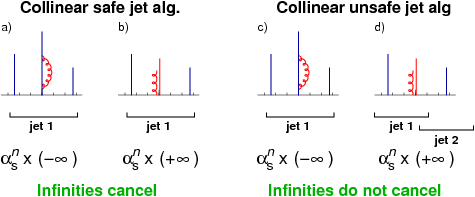
\includegraphics[width=1.0\textwidth]{images/collinear_safe.png}
\caption[Collinear safe ilustration]{A description of collinear safe and an collinear unsafe algorithm. Here we have two situations that must be treated on equal grounds due to theoretical reasons and might not be so due to the choice of jet algorithm. Figure from \cite{salam_towards_2010}}
\label{collinear_safe}
\end{figure}

Another type of problem that might occur is due to soft radiation. This situation can be seen in Figure \ref{infrared_safe}. As before, we have two final states that must be treated on the same ground, from the theoretical perspective. But the algorithm might not do so. It can happen because the extra particle seen in red in the Figure might act as a new seed and cluster two jets into one. Algorithms that succeed in avoiding this merging are called infrared safe.

\begin{figure}
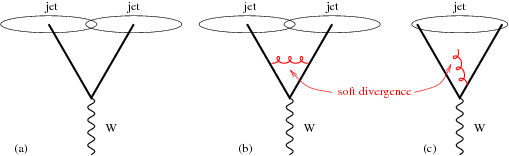
\includegraphics[width=1.0\textwidth]{images/infrared_safe.png}
\caption[Collinear safe ilustration]{A description of infrared safe and an infrared unsafe algorithm. Here we have two situations that must be treated on equal grounds due to theoretical reasons and might not be so due to the choice of jet algorithm. Figure from \cite{salam_towards_2010}}
\label{infrared_safe}
\end{figure}

One of the algorithms that satisfy to a good extent these criteria is the anti-kt algorithm\citep{cacciari_fastjet_2012}. The anti-kt algorithm belongs to a broader class called the recombination algorithms. The members of this class are all based on the idea of a distance defined between every pair of particles being analyzed. If the distance is smaller than the distance of another particle to the beam, the particles are combined. This process is repeated until no single pair satisfies the condition and one ends up with a set of jets of the event. At this stage, further cuts might be done in the rapidity or the $p_t$ of the jet. The distance used in the anti-kt algorithm is defined by the following equation:

\begin{equation} \label{jet_alg}
d_{ij} = \min (p_{t i}^{2p},p_{t j}^{2p}) \frac{\Delta R_{ij}}{R}
\end{equation}

Where $R$ is a parameter that is defined at each analysis. For $p=-1$\footnote{The value $p=1$ corresponds to the $k_t$ algorithm and $p=0$ to the Cambridge-Achen. See \cite{salam_towards_2010} for further details}. Where:

\begin{equation} \label{delta_r}
\Delta R_{ij} = \sqrt{ (\eta_i - \eta_j)^2 + (\phi_i - \phi_j)^2 }
\end{equation}

A distance to the beam axis is also defined:

\begin{equation}
d_i = p_{ti}^{-2}
\end{equation}

From all the $d_{ij}$ and $d_i$ the minimum value is chosen. If it is $d_i$ then this particle is removed from the list and called a jet. Otherwise, it is a distance $d_{ij}$, the $i$ and $j$ particles are combined. The process goes on iteratively until a final list of jet candidates is left. The recombination of the particles is performed using the $E$ scheme, or 4-momentum scheme, which means particles are combined by adding their 4-momenta.

\mysubsection{Background subtraction}

An extra difficulty arises when trying to perform jet analysis in heavy-ion collisions due to the background contamination, called the Underlying Event (UE). The UE corresponds to the soft particles that come from the radiation of the freeze-out surface and are mainly explained through hydrodynamics. When one is trying to cluster jets, experimentally, one must subtract this background in other to make comparisons with theory.
\par
In JEWEL, the recoiling scattering centers can be kept and included in the final state of the events. Whenever there is an elastic collision during the parton propagation, the distinction between the 4 momentum that is part of the jet and the 4 momentum that is part of the medium is spoiled. To address this problem, the scattering centers kept by JEWEL are used to subtract this 4 momenta from the final state.
\par
Following \cite{zapp_geometrical_2014}, the background subtraction is performed by the use of ghost particles. These particles are inserted into the final state with very low $p_T$ and the same direction as the four-momentum assigned to the scattering center. Particles are then classified as background if they satisfy the following condition:

\begin{equation}
\Delta R_{ij} < 1 \cdot 10^{-5}
\end{equation}

Where $\Delta R_{ij}$ is the distance to the closest ghost particle (see Equation \eqref{delta_r}). The list compiled by evaluating this condition is then subtracted according to each observable. In the case of jet girth, for instance, the particles deemed to be background are removed from the jet constituents list and thus do not participate of the observable calculation. In the case of jet dispersion, we used:

\begin{equation}
p_T^D = \frac{\sqrt{ \sum_{\rm particles} {p_t}^2 - \sum_{\rm background} {p_t}^2 }}{p_{t,corrected}^{jet}}
\end{equation}

For the jet mass, a correction of the jet four-momentum comes automatically when removing the background from the list of particles.

\mysection{Jet Observables}

Although the main idea of a jet is to reconstruct the basic partonic kinematics of a hard scattering, there are a lot of things that can be investigated with a jet. This is since the jet has more information than a single particle. One can study its shape and structure to find radiation patterns and non-perturbative dynamics. In the present work, the main idea is to look for radiation patterns. Here we define the observables that can characterize the jets used in this work.

\mysubsection{Girth}

The generalized angularities for the jet constituents are defined as:

\begin{equation} \label{gen_ang}
\lambda_{\beta}^{\kappa} = \sum_i \left( \frac{p_{T,i}}{p_{T,jet}} \right)^\kappa \left( \frac{\Delta R_{jet,i}}{R} \right)^\beta
\end{equation}

Where $\kappa$, $\beta$ and $R$ are parameters chosen at each analysis. $\Delta R_{jet,i}$ is the angular distance between jet and constituent $i$. Girth is related to the angular opening of the jet. The idea is to pick the first order moment in angular distribution with the constituents $p_T$ as weights. This means picking $\beta=\kappa=1$. Girth is defined by:

\begin{equation}
g = \sum_{\rm constituents} \frac{p_t}{p_t^{jet}} \Delta R_{i,jet}
\end{equation}

Where $\Delta R_{i,jet}$ is calculated according to \eqref{delta_r} and the sum is taken on the constituents of the jet. Its possible values lie in the $\left[ 0,1 \right]$ interval. Girth is also known in some collaborations as jet width. Unlike the jet mass, it depends linearly on the transverse momentum of the constituent particles. Therefore, it is more sensitive to softer fragmentation.

\mysubsection{Dispersion}

This observable measures the \emph{hardness} of the fragmentation of the jet. This means that it will have a large value if the jet $p_t$ is distributed in fewer particles, and smaller values if the $p_t$ is distributed in a larger number of particles. Its definition is given by the equation:

\begin{equation}
p_T^D = \frac{\sqrt{ \sum_{\rm constituents} {p_{t,i}}^2 }}{p_t^{jet}}
\end{equation}

Where the sum is taken on the constituents of the jet. It corresponds to $\kappa=2$ and $\beta=0$ in Equation \eqref{gen_ang}. It can be seen from its definition that the possible values lie in the $\left[0 , 1 \right]$ interval. Values close to one will correspond to the extreme case of the jet transverse momentum being distributed in one or two constituents and one of them carries most of its momentum. The opposite limit corresponds to the jet transverse momentum being distributed almost equally on a high number of constituents.

\mysubsection{Jet Mass}

The jet mass is a observable that is constructed from the jet four-momentum in the usual Lorentz formalism. The definition is:

\begin{equation}
M_J = \sqrt{ \left( \sum_{\rm particles} {\rm E} \right)^2 - \left( \sum_{\rm particles} {\rm \overrightarrow{p}} \right)^2 }
\end{equation}

It can be seen, in the RHS of the above equation that this observable is sensitive to the collimation of the jet. This can be observed by noting that, inside the square root, there is a scalar sum and a vector sum, where vector sum depends on the angular separation of the constituents. The broader the jet, the smaller the jet mass. And the impact of each constituent particle in this observable depends on the squared transverse momentum. This increases the impact of the harder constituents of the jet.


%\mysubsection{SoftDrop}

%There is another interesting observable regarding the substructure of a jet that is the fraction of $p_T$ carried by the softest of the two proto-jets forming a jet. To find this quantity, one must first apply the anti-kt algorithm to an event. After that, one runs the C/A algorithm just on the constituents of a given jet until there are two proto-jets. If they satisfy the SoftDrop condition:

%\begin{equation}
%z = \frac{\min (p_T^A, p_T^B)}{p_T^A + p_T^B} \Delta R^{\beta} > z_g
%\end{equation}

%Then $z$ is counted on a histogram, else, the highest $p_T$ jet is inserted back into the C/A and the process is repeated. This observable tries to find the first and hardest splitting that the parton that gave birth to the jet went through.

\mysubsection{Azimuthal anisotropy $v_2$}

The azimuthal anisotropy for a given observable comes from the idea of expanding a given spectrum in the following form:

\begin{equation}
\frac{{\rm dN}}{{\rm d}^2p_T {\rm d}\eta {\rm d}\phi } = \frac{{\rm dN}}{{\rm d}^2p_T {\rm d}\eta } \left[ 1 + \sum_n 2 v_n \cos \left( n ( \phi - \Psi_{\rm RP} ) \right) \right]
\end{equation}

Where $\Psi_{\rm RP}$ is the reaction plane angle. The coefficients $v_n$ are adjusted and represent the lack of cylindrical symmetry of the spectra. $v_2$ is called the azimuthal anisotropy coefficient and $v_3$ is the triangular flow. They usually reflect the geometry of the initial conditions set by the early dynamics, before the hydro phase. The harder problem in the measurement of these quantities is the determination of the reaction plane, which is random. Usually, it is calculated by adjusting the above formula with the distribution in $\phi$ of the observed particles in an event. The $v_2$ coefficient is related to the ellipticity of the initial conditions for the hydro expansion. As can be seen in Figure \ref{v2}, it comes from the shape of the overlap zone of the colliding nuclei.

\mysection{Grid validation}

As a validation for the grid method implemented in this work, we show here a comparison between observables calculated with JEWEL in its default configuration and with the grid method implemented here. In Figure \ref{grid_jetpt_validation} we can see the jet $p_T$ spectrum for both cases. And in Figure \ref{grid_default} we can see a ratio plot of both spectra. Within the statistical uncertainty calculated for the Monte Carlo, we can see that they both agree. This result shows that errors inserted due to interpolation of the grid do not affect this observable.

\begin{figure}
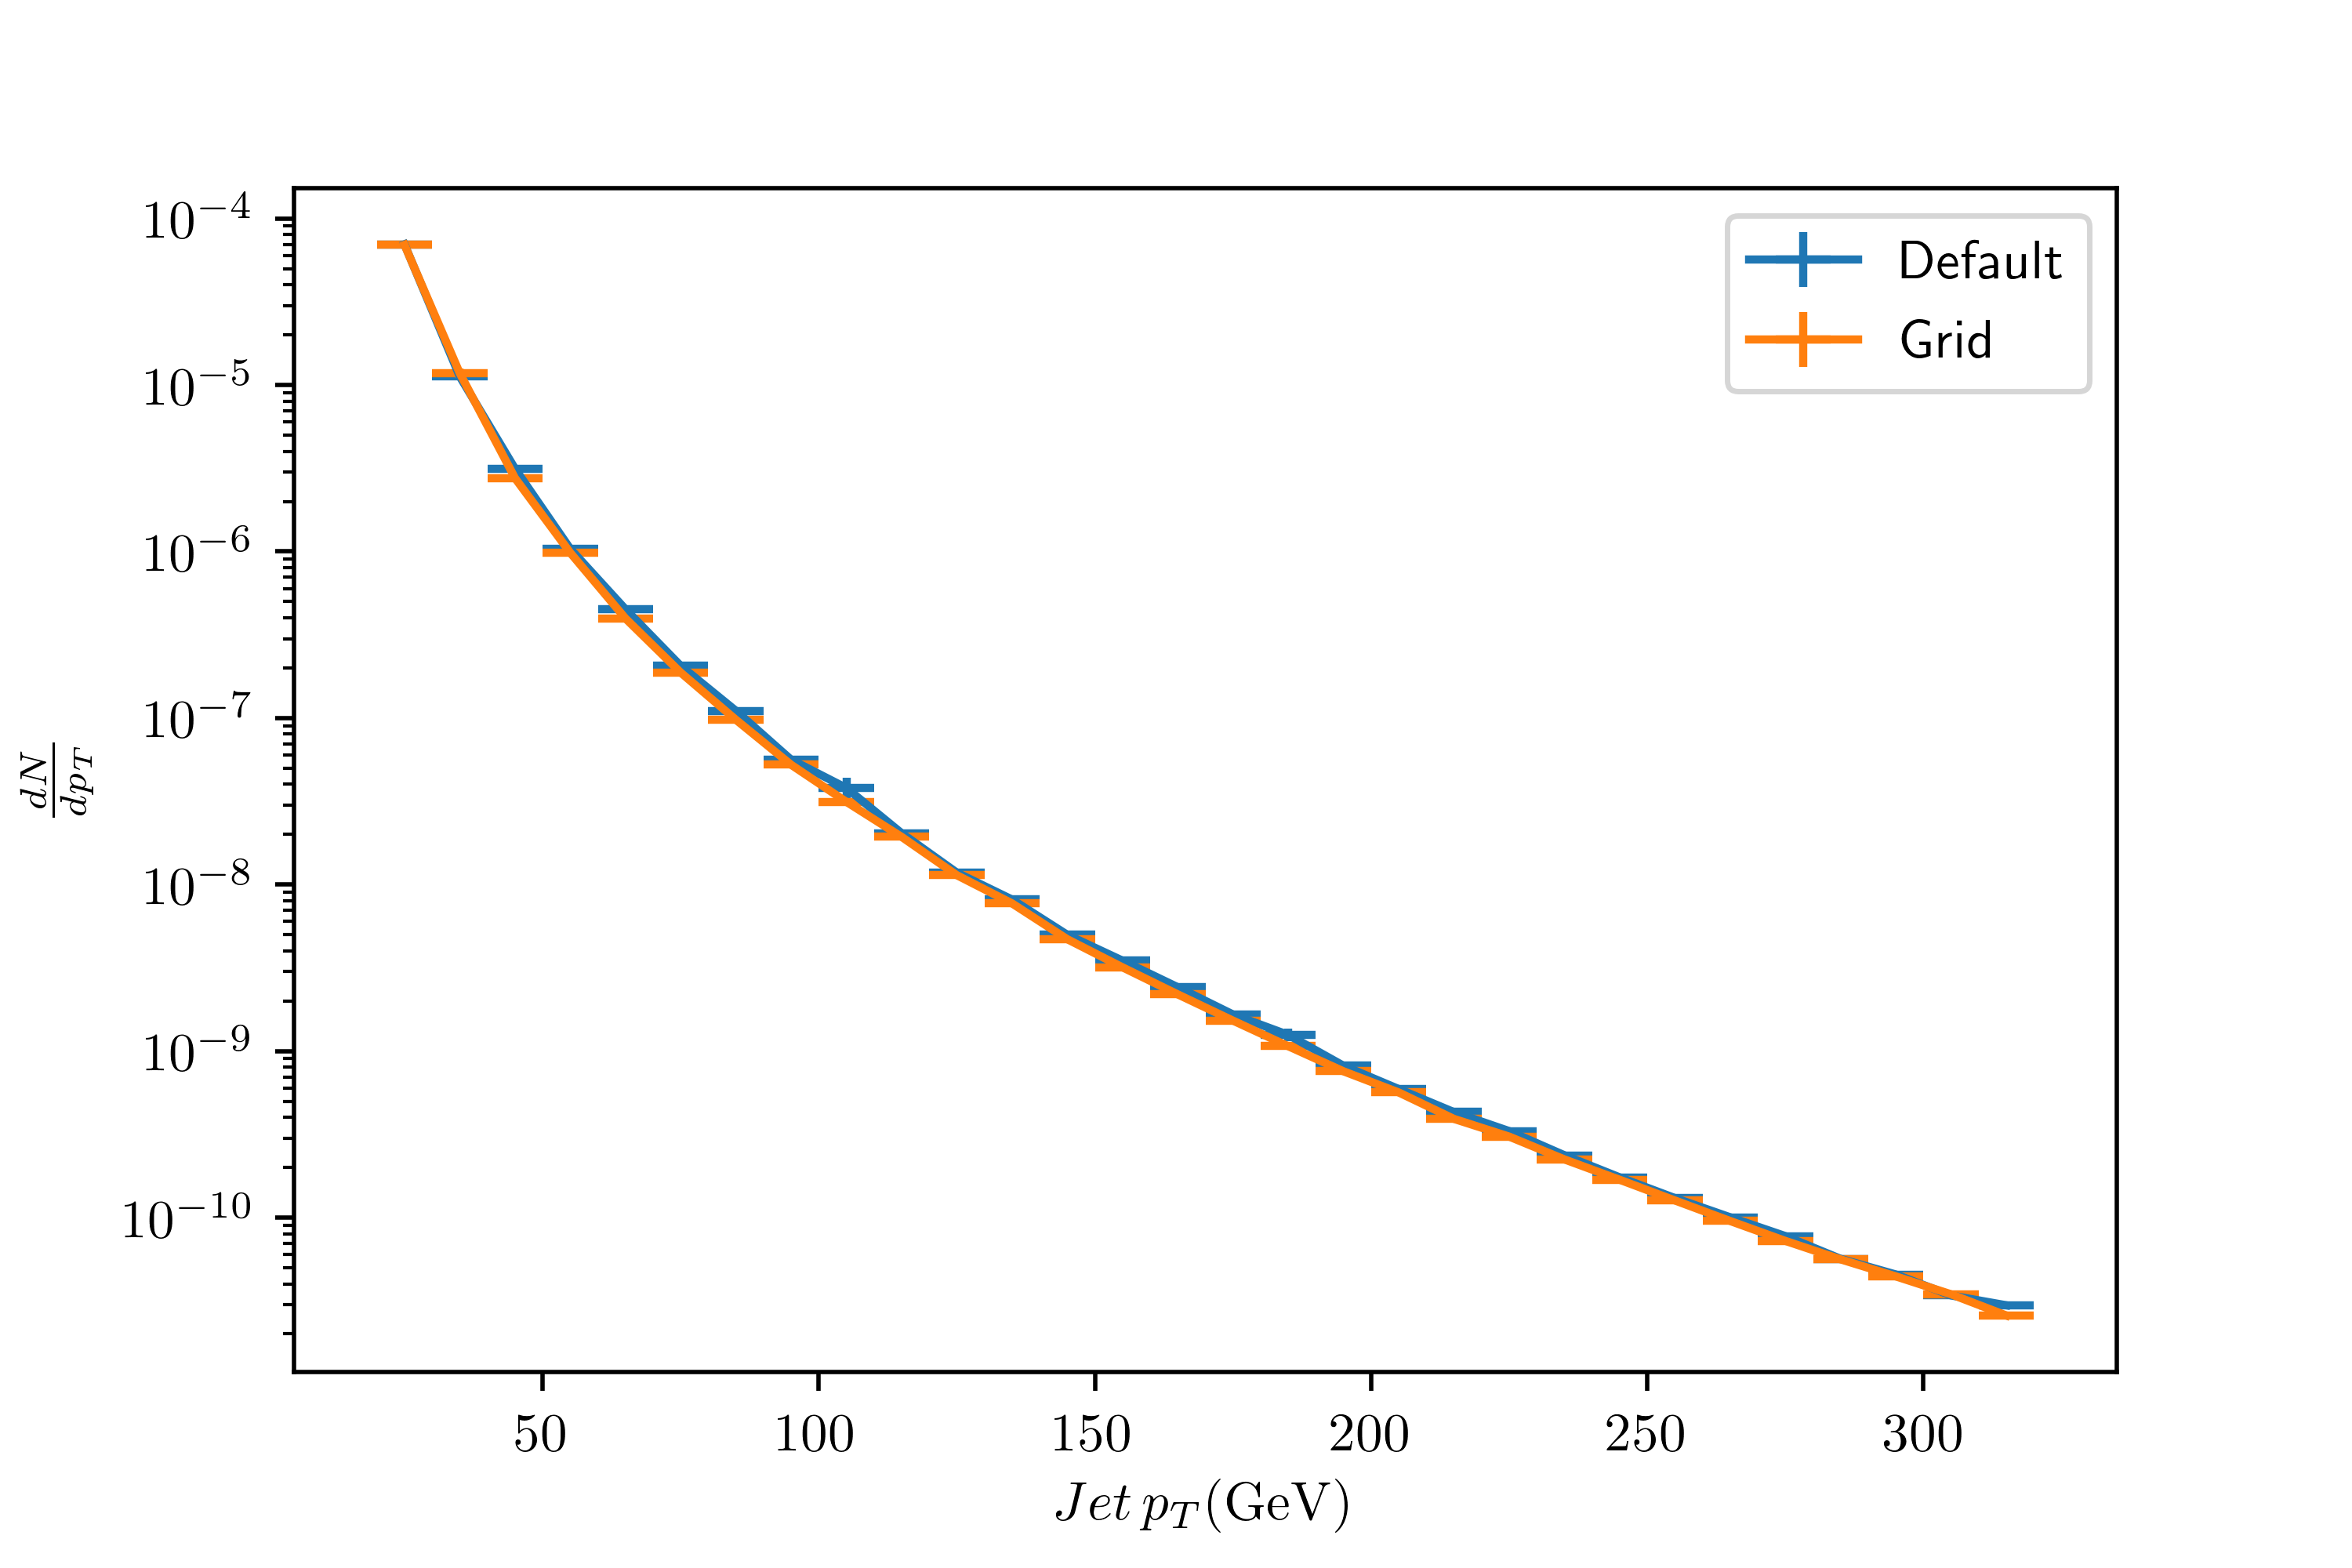
\includegraphics[width=0.7\textwidth]{images/grid_jetpt_validation.png}
\caption[Jet $p_T$ for Grid validation.]{Jet $p_T$ for Grid validation.}
\label{grid_jetpt_validation}
\end{figure}

\begin{figure}
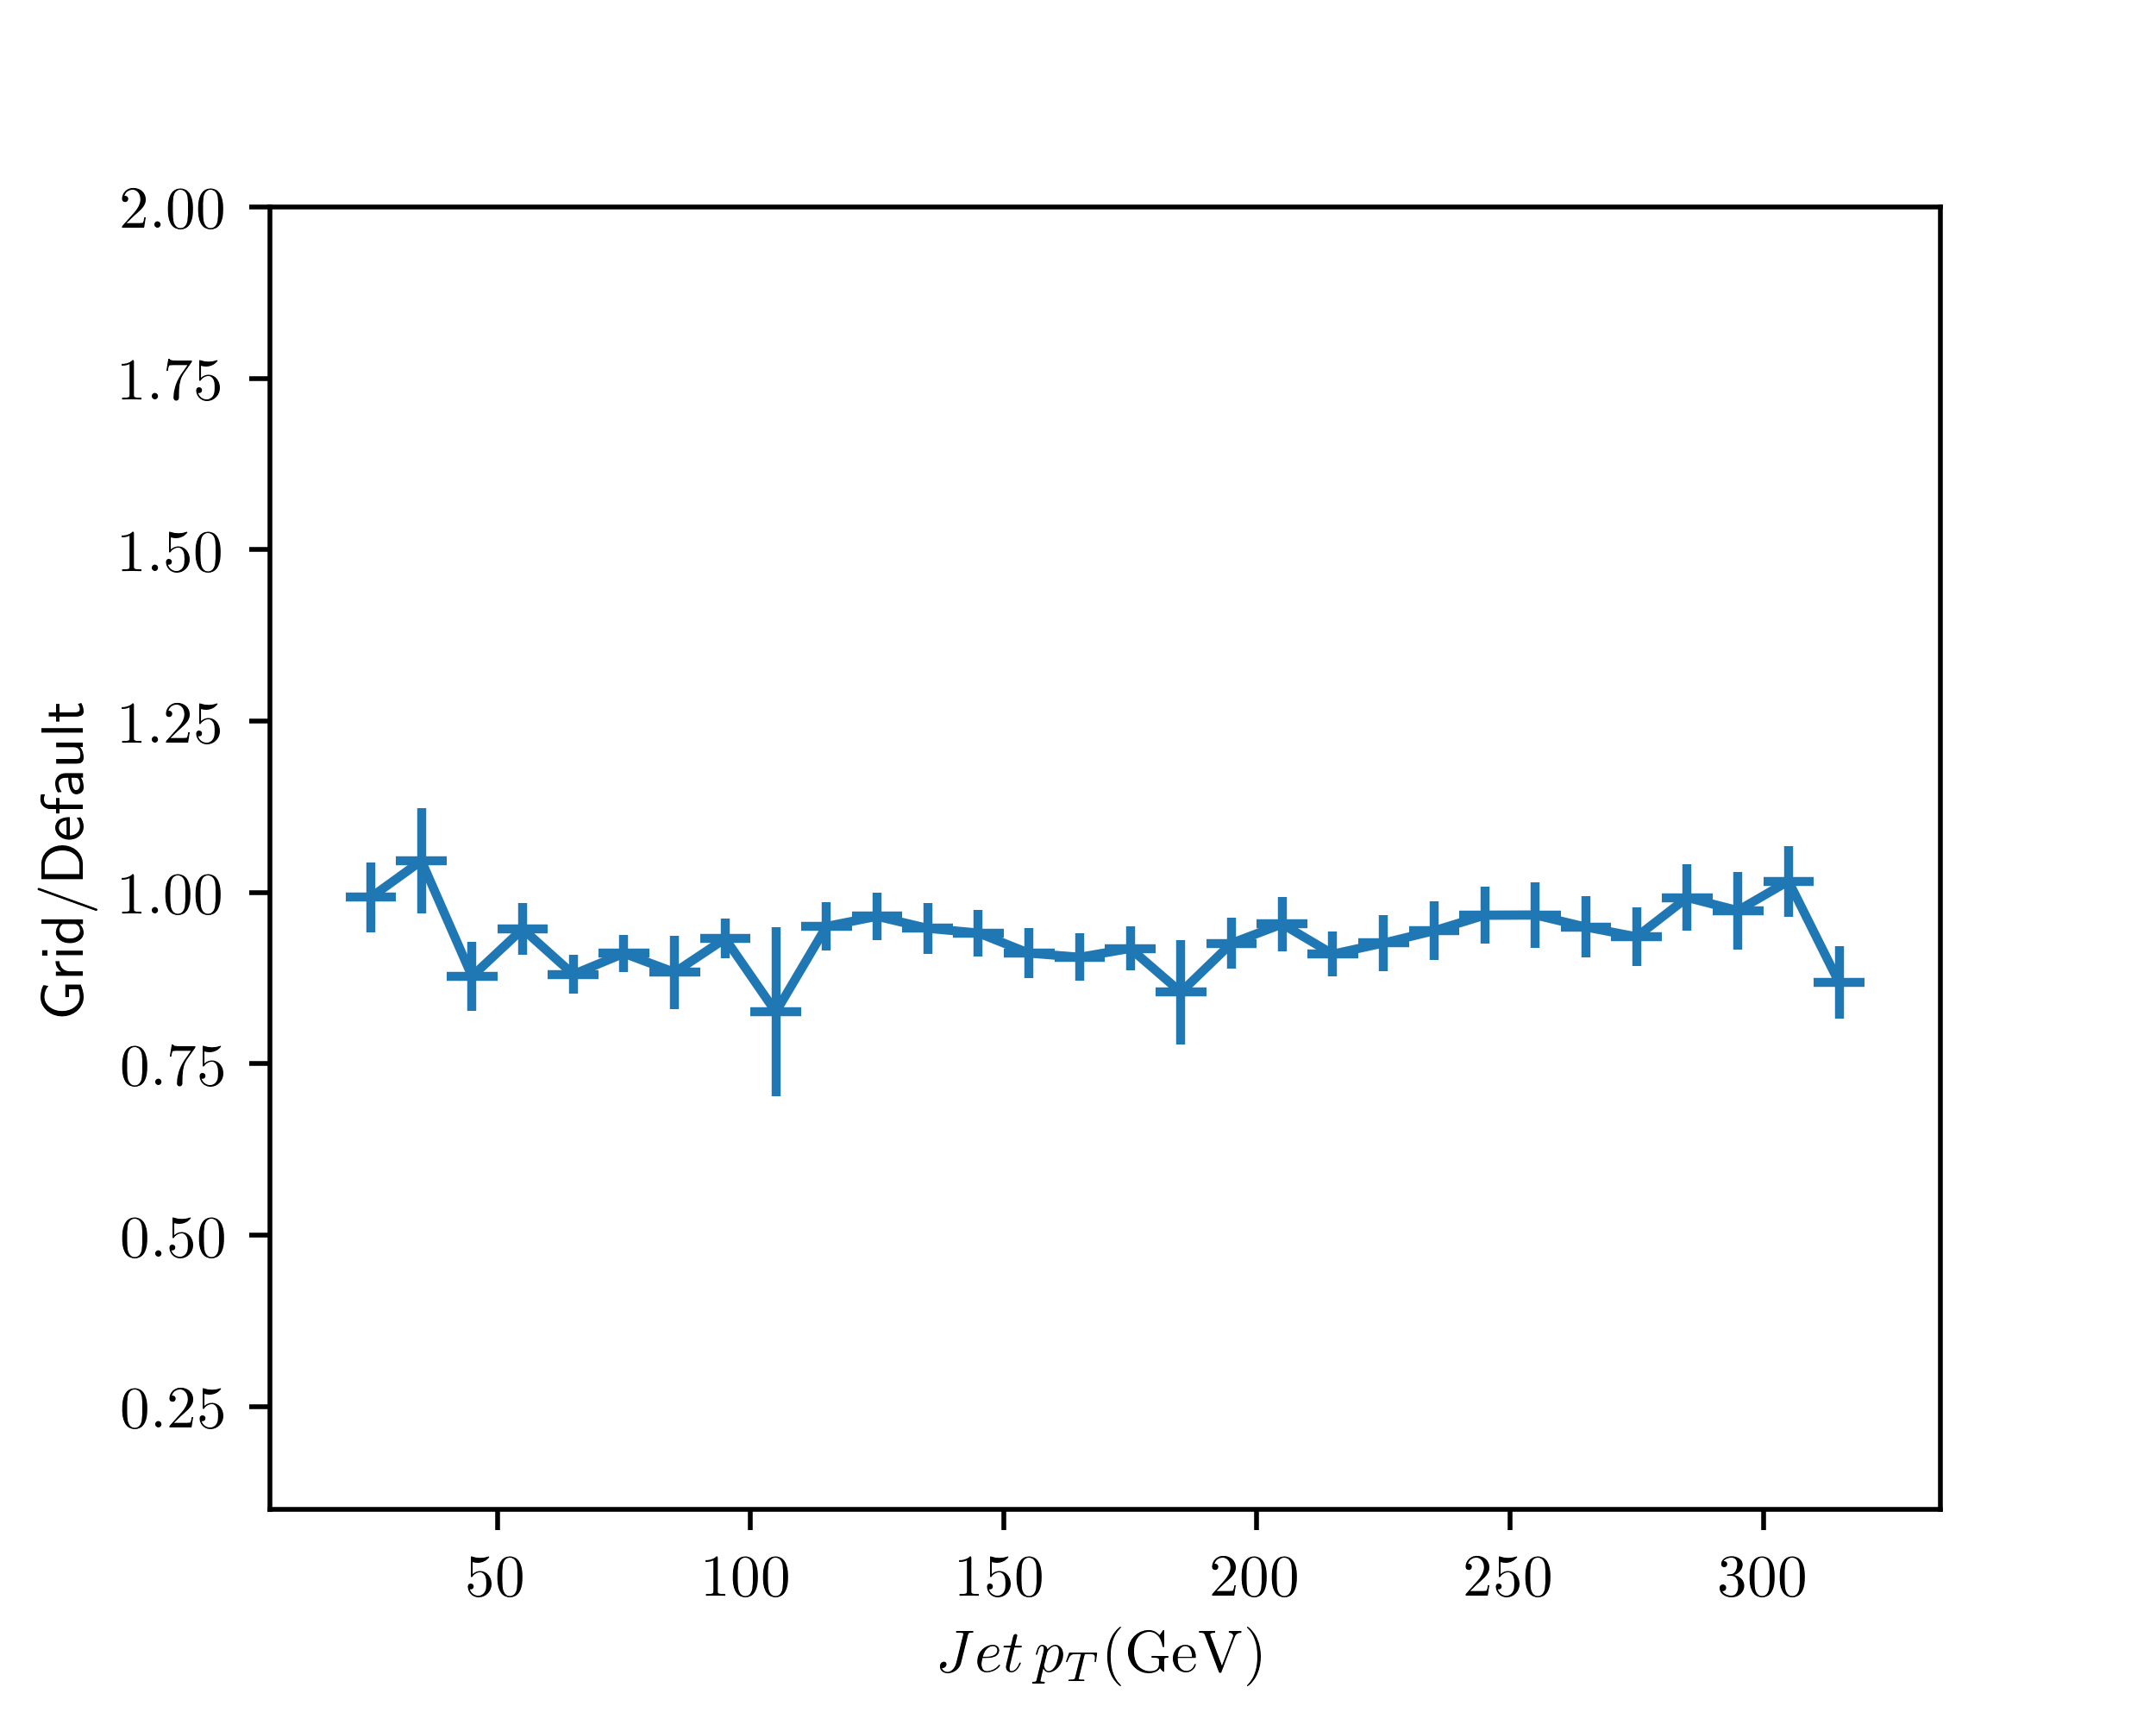
\includegraphics[width=0.7\textwidth]{images/grid_default_jetpt.png}
\caption[Grid/Default for jet $p_T$]{Grid/Default for jet $p_T$}
\label{grid_default}
\end{figure}

For the case jet mass we can see a plot of the spectra and a ratio plot on Figures \ref{grid_jetmass_validation} and \ref{grid_default_jetmass}, respectively. The mass has an error of $25\%$ in only one bin, but the rest of the bins is well controlled within the uncertainties. This shows that both methods agree. The peak and width of the distribution are well reproduced.

\begin{figure}
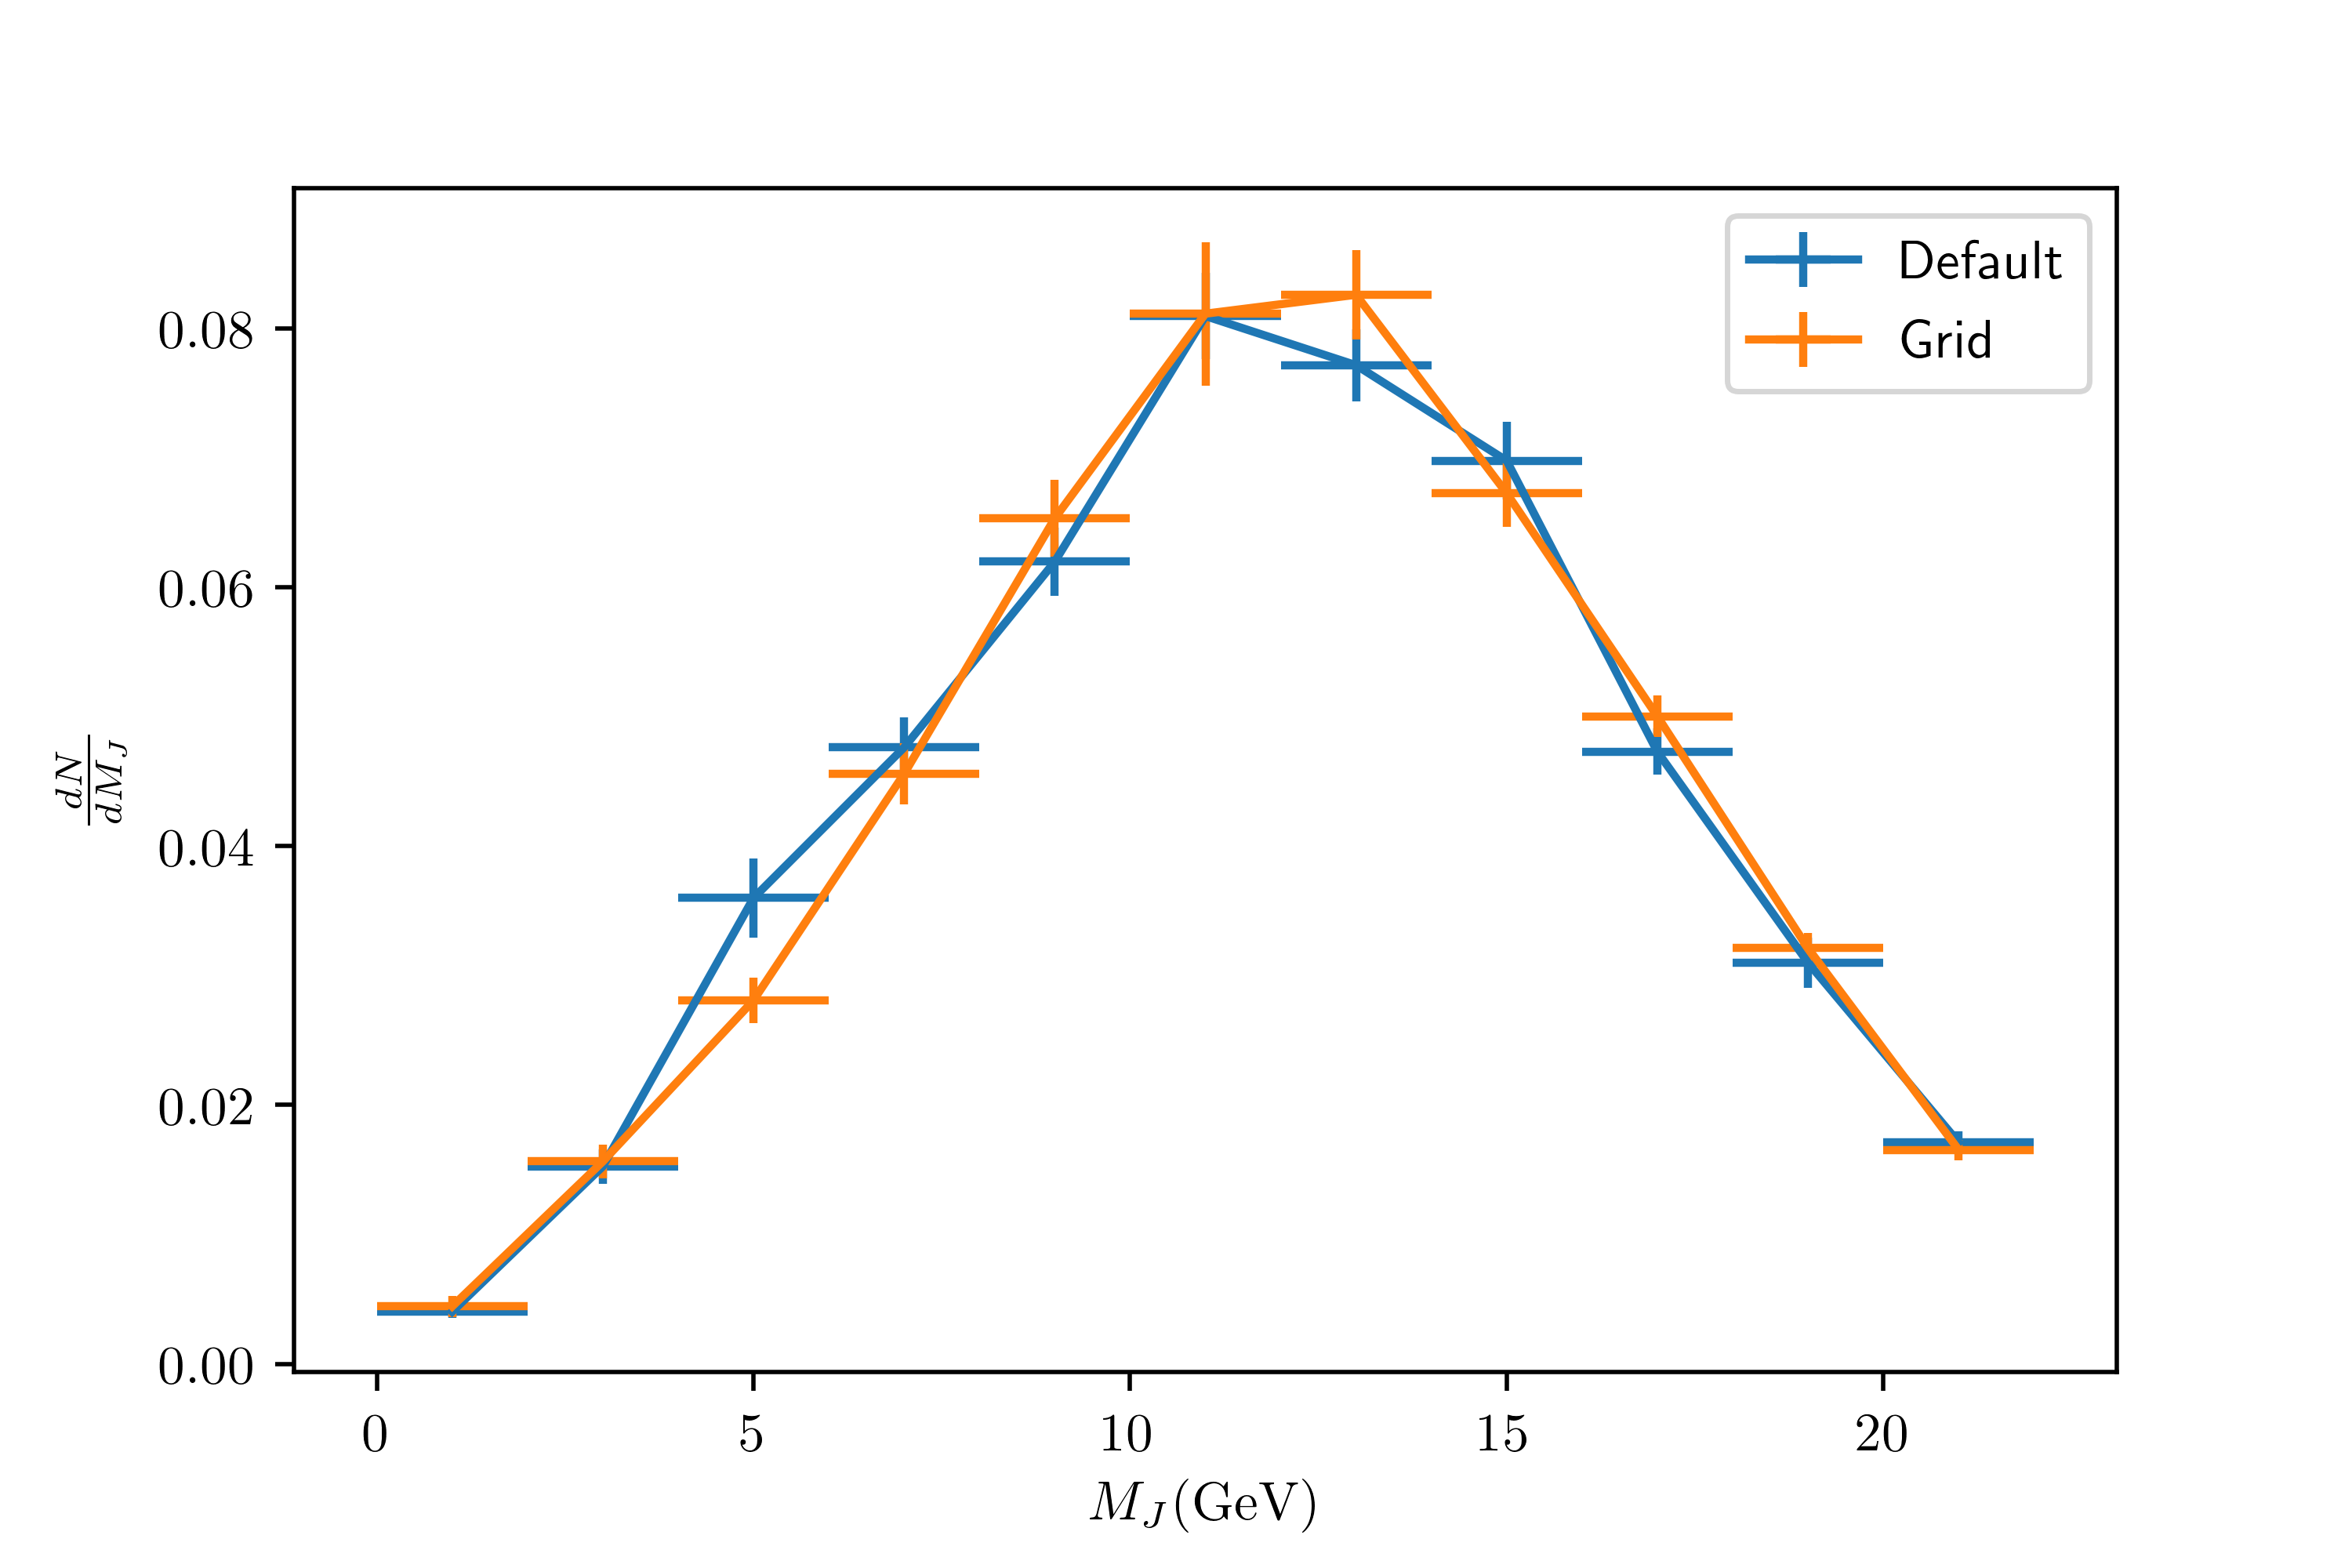
\includegraphics[width=0.7\textwidth]{images/grid_mass_validation.png}
\caption[Jet Mass for Grid validation.]{Jet Mass for Grid validation.}
\label{grid_jetmass_validation}
\end{figure}

\begin{figure}
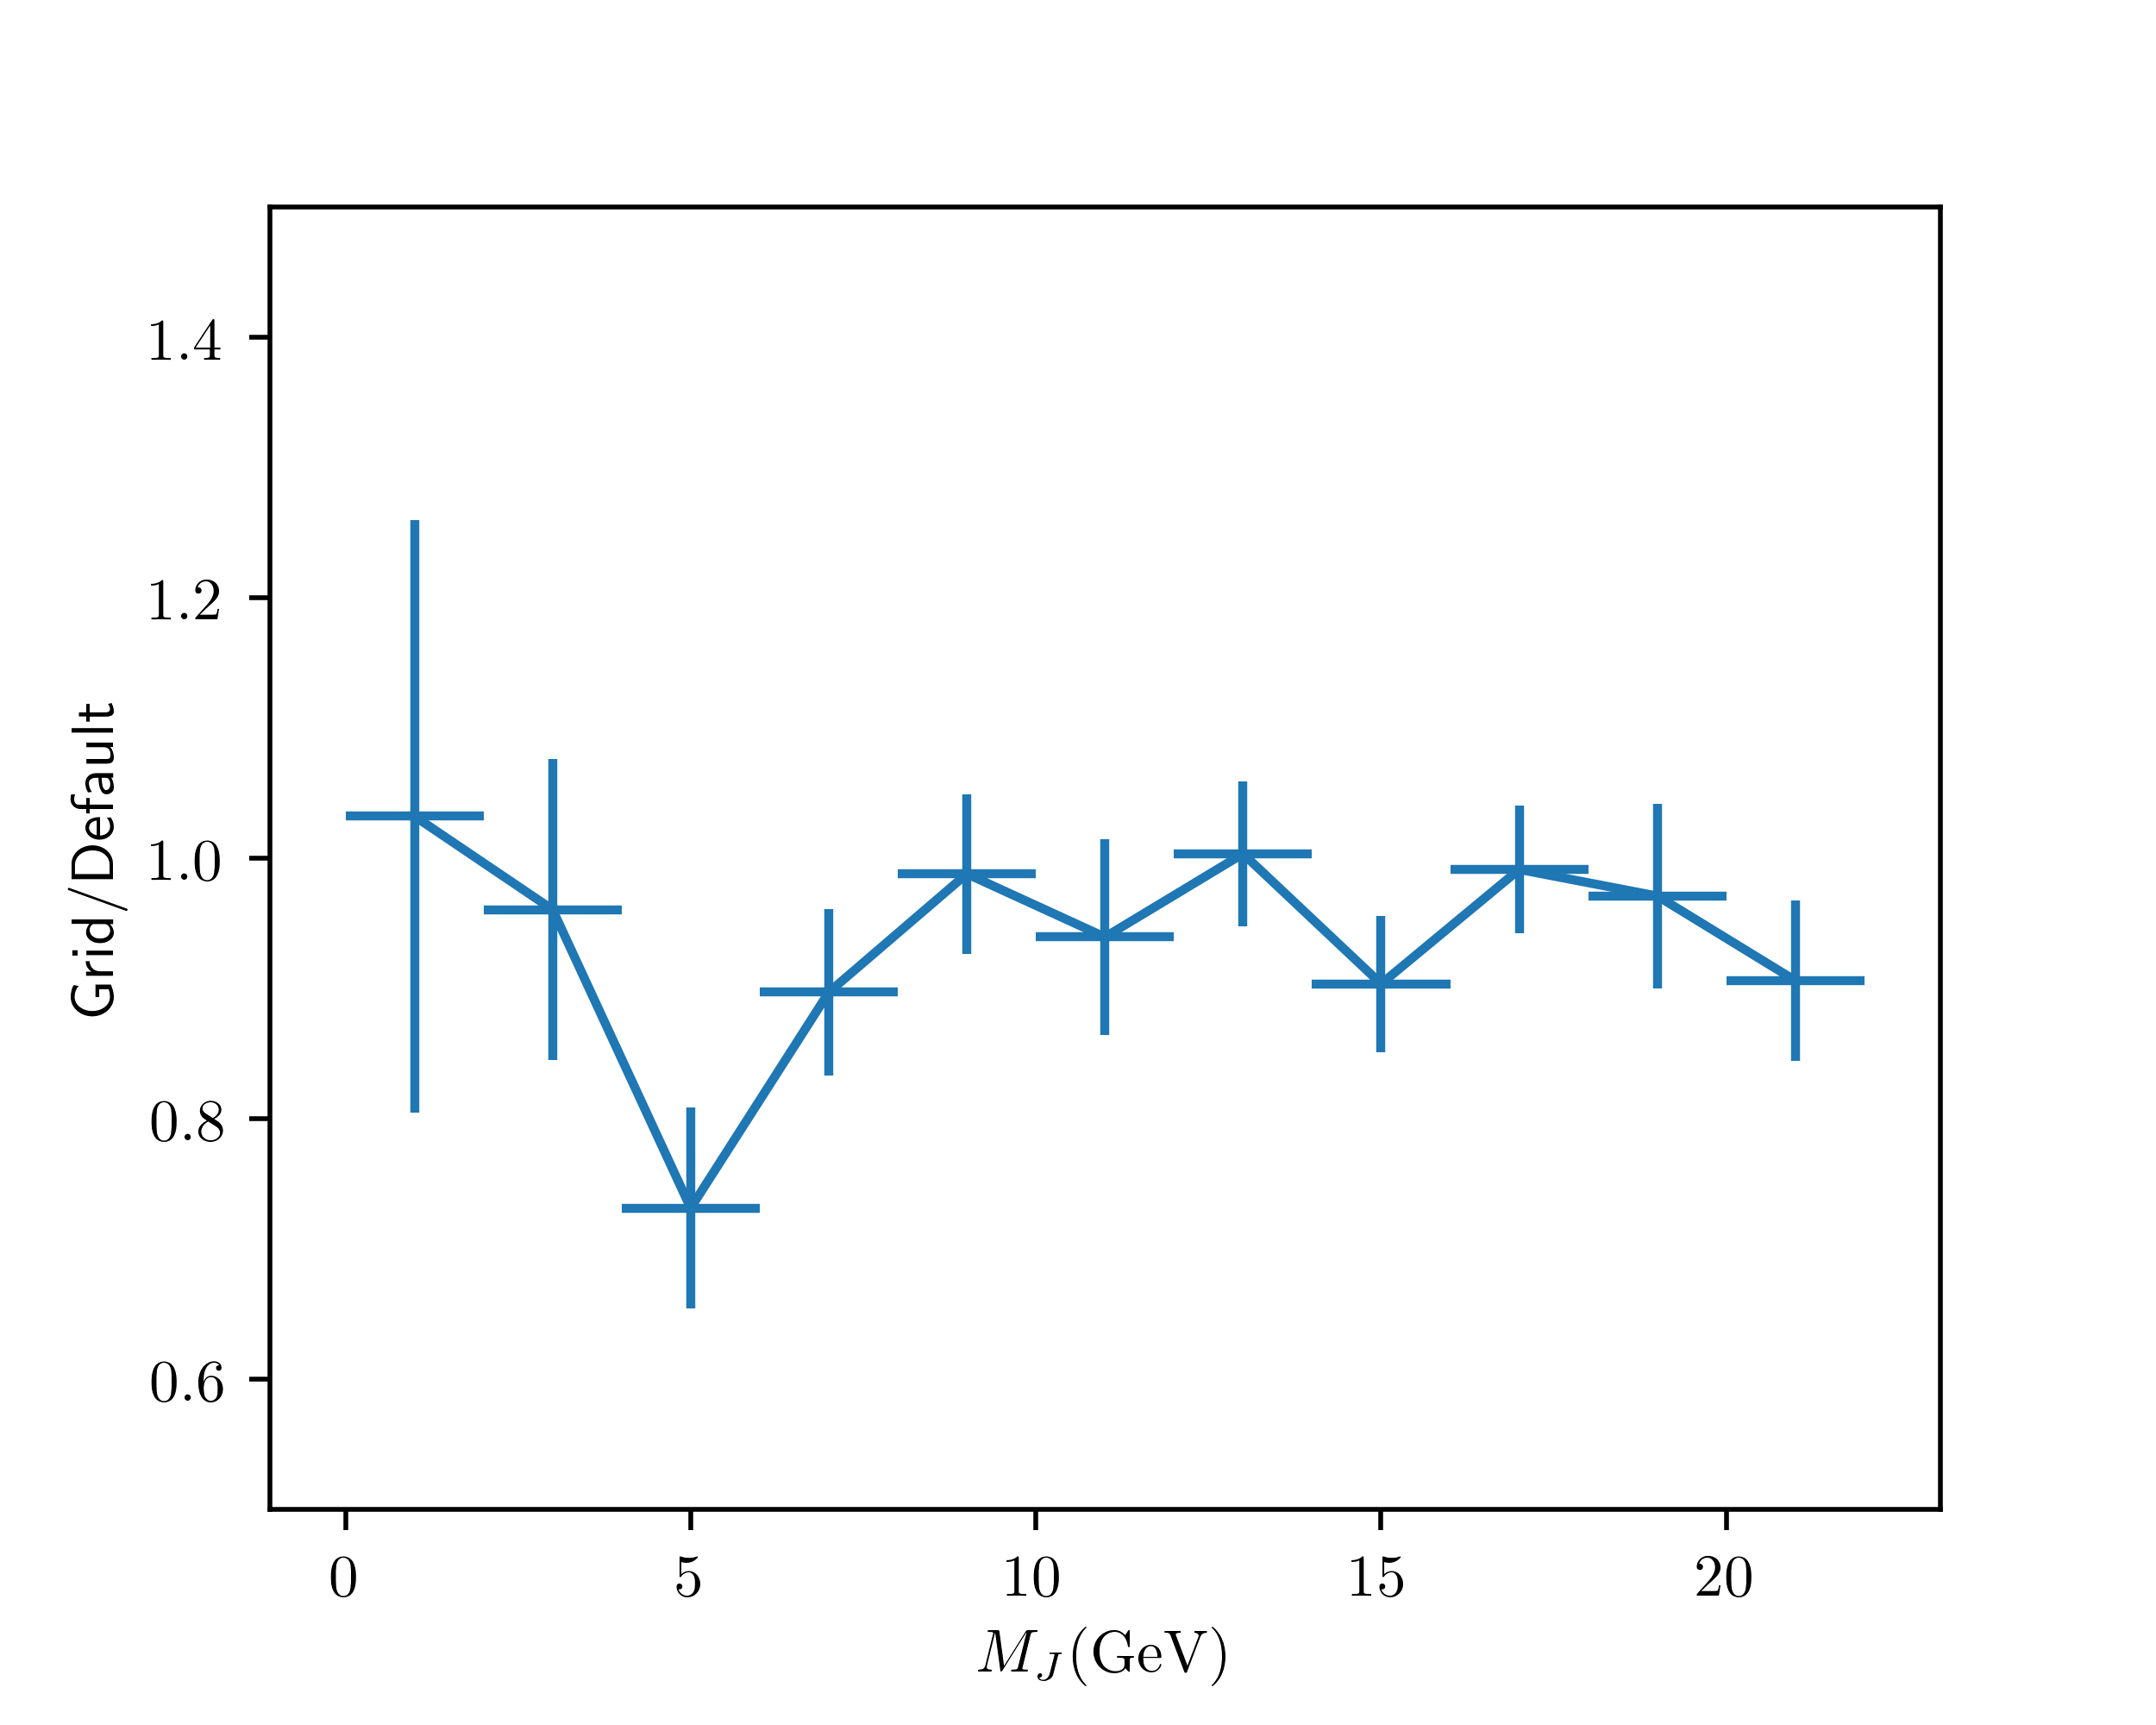
\includegraphics[width=0.7\textwidth]{images/grid_default_mass.png}
\caption[Grid/Default for jet mass]{Grid/Default for jet mass}
\label{grid_default_jetmass}
\end{figure}

On Figures \ref{grid_girth_validation} and \ref{grid_default_girth} we can see the plots for the jet girth for both cases and also a ratio plot. The qualitative behavior is reproduced. Within the uncertainties, the data of both methods agree. The peak and width of the distribution are well reproduced.

\begin{figure}
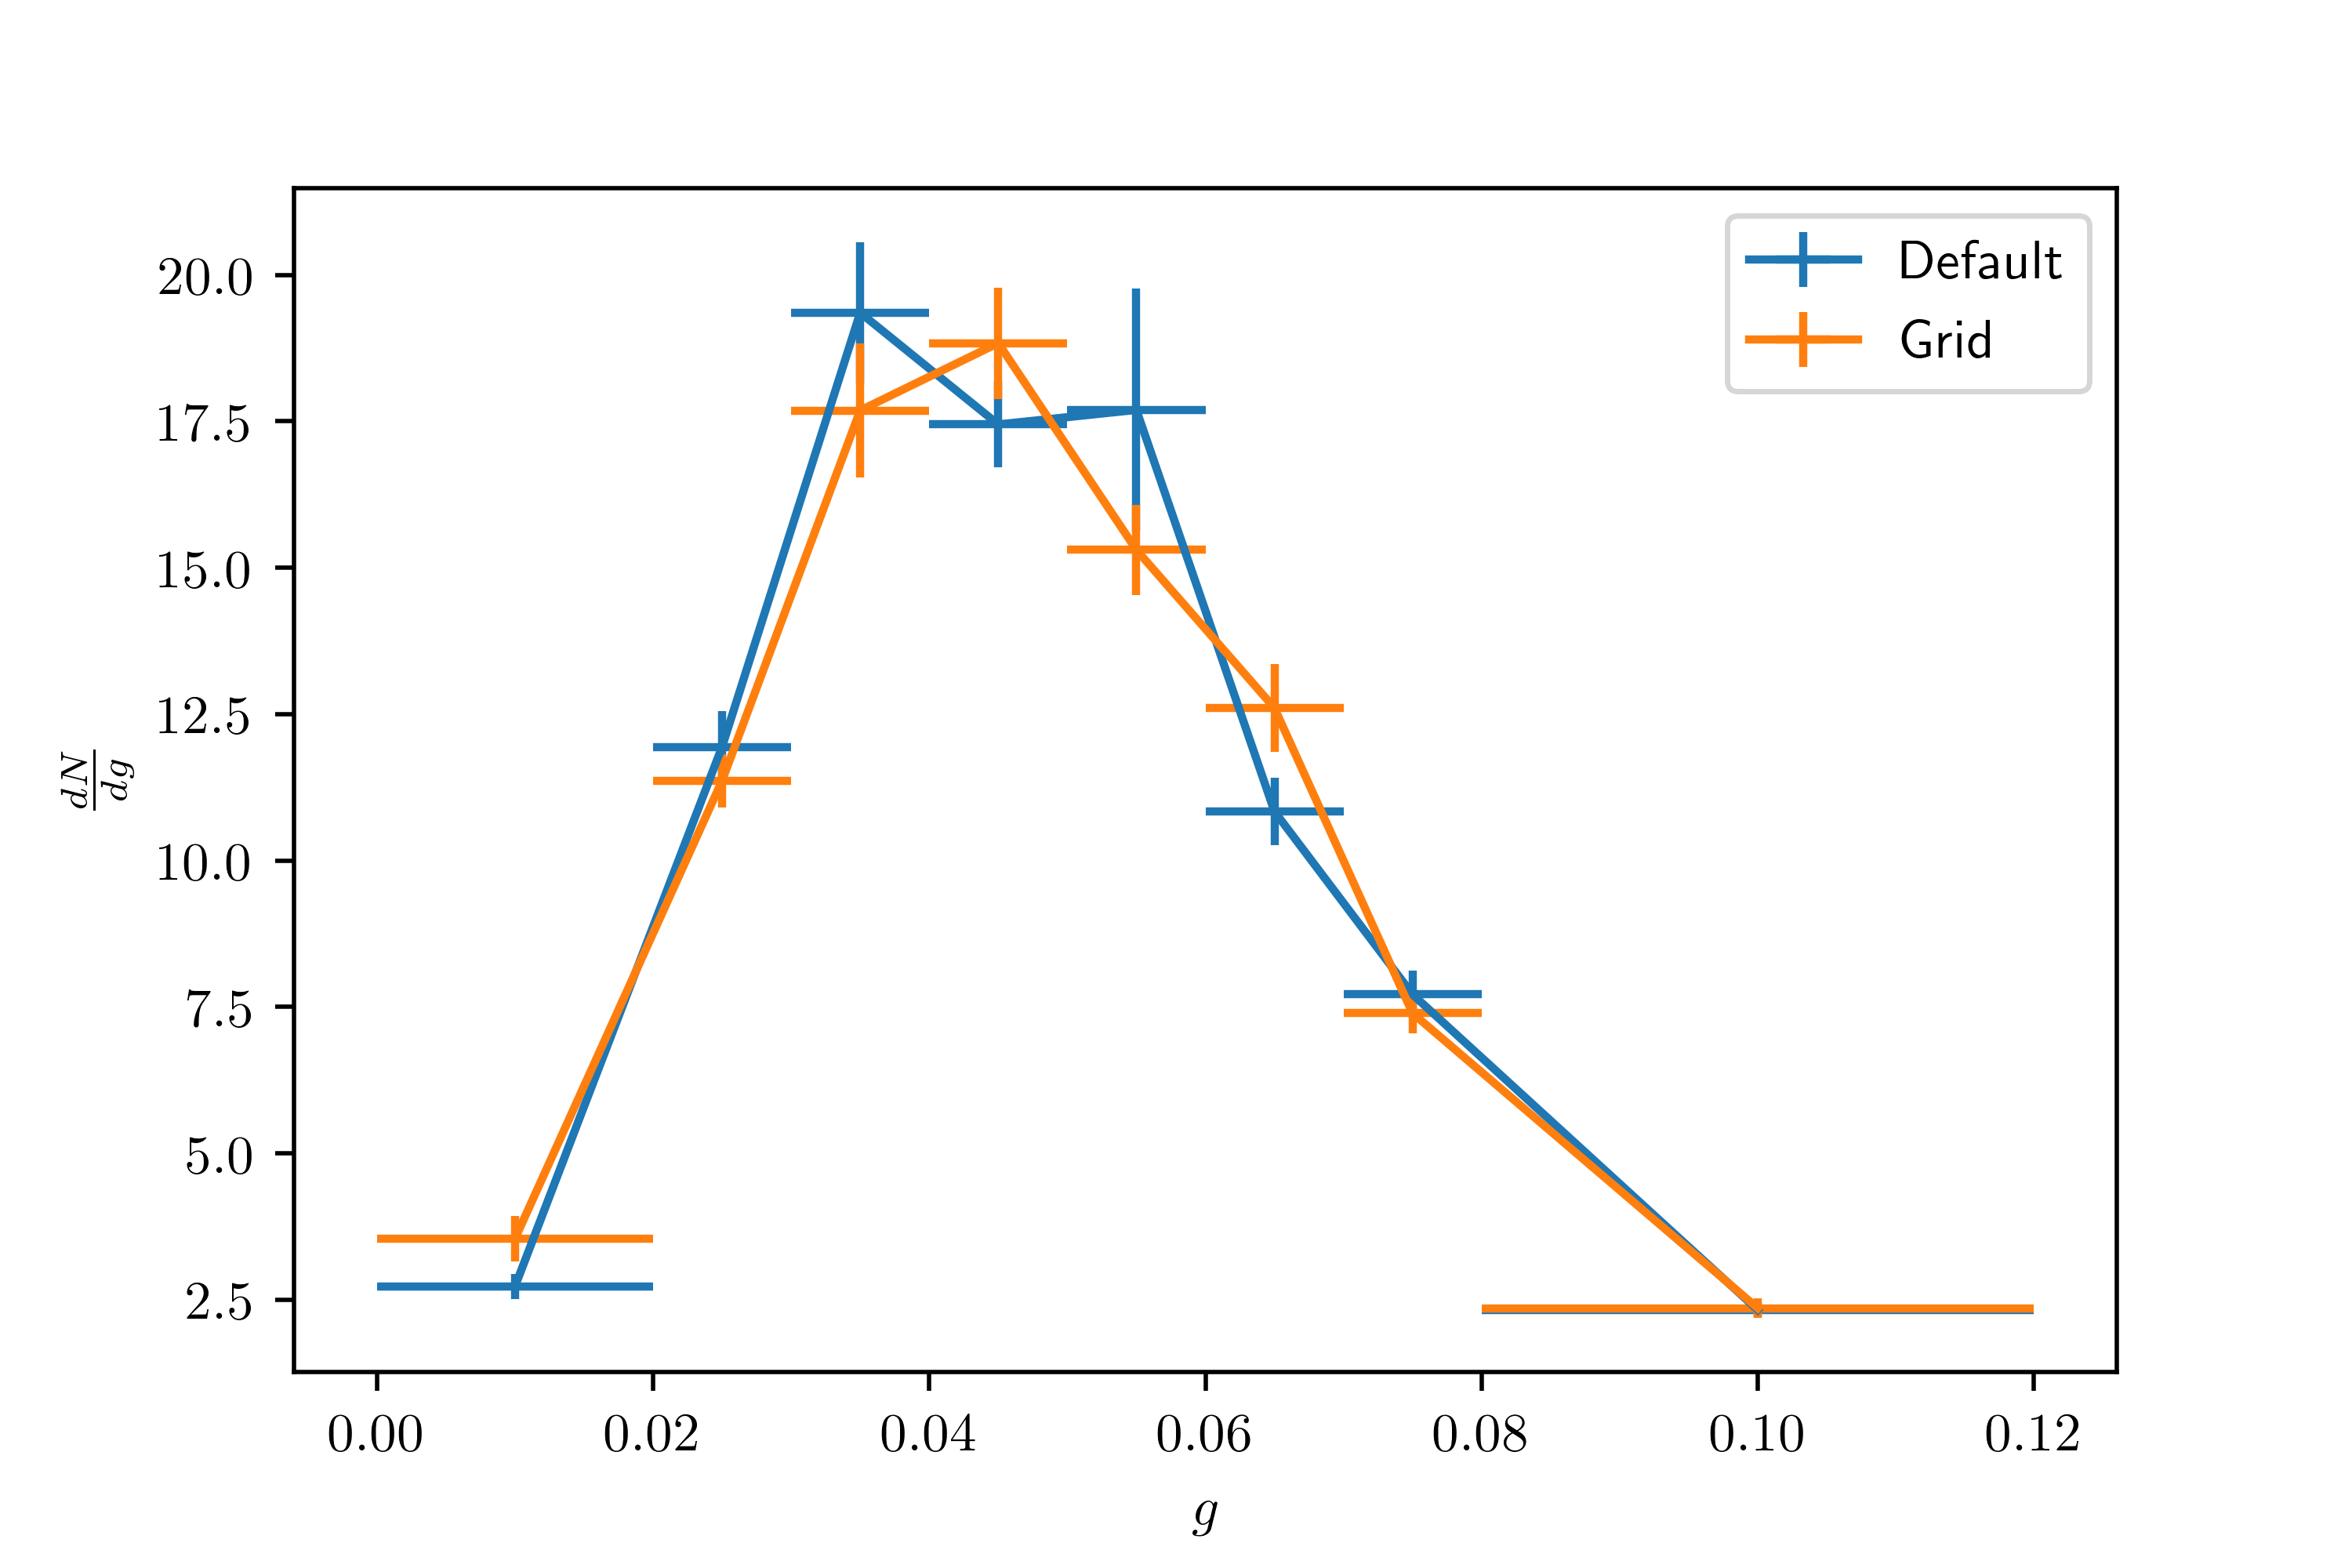
\includegraphics[width=0.7\textwidth]{images/grid_girth_validation.png}
\caption[Jet Girth for Grid validation.]{Jet Girth for Grid validation.}
\label{grid_girth_validation}
\end{figure}

\begin{figure}
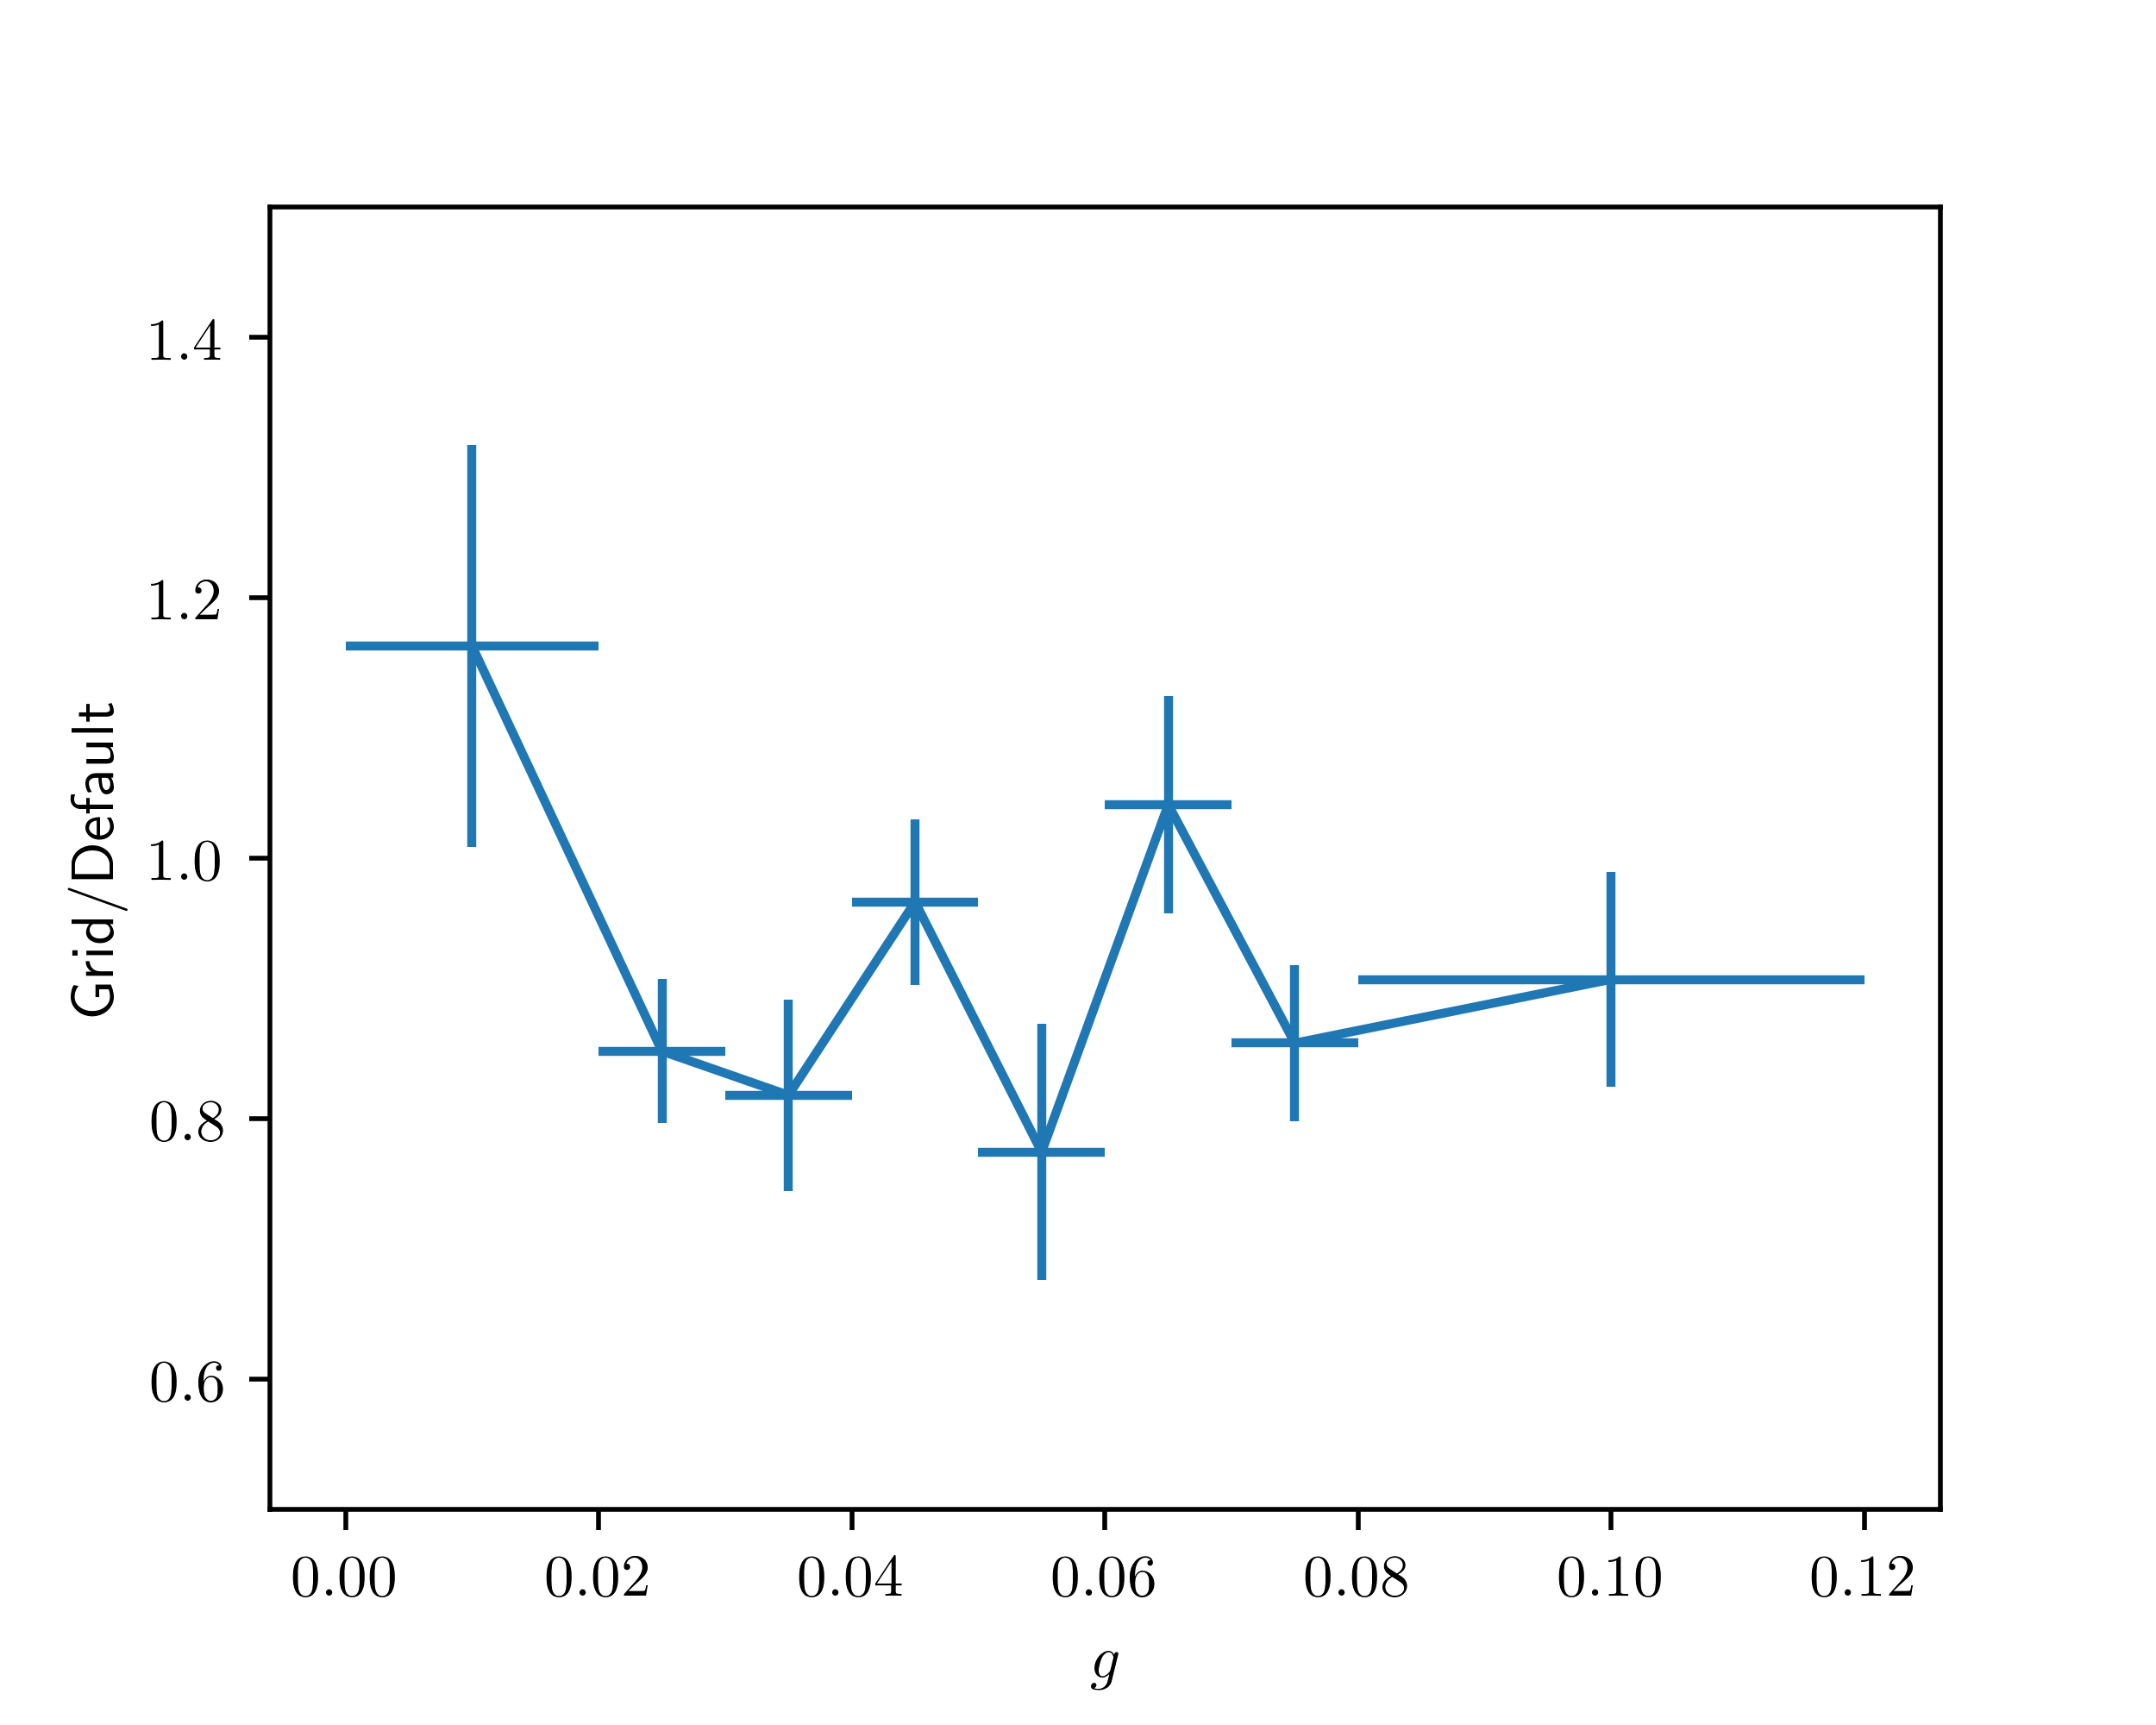
\includegraphics[width=0.7\textwidth]{images/grid_default_girth.png}
\caption[Grid/Default for jet girth]{Grid/Default for jet girth}
\label{grid_default_girth}
\end{figure}

On Figures \ref{grid_dispersion_validation} and \ref{grid_default_girth} we can see the plots for the jet $p_T^D$ for both cases and also a ratio plot. The qualitative behavior is reproduced. Within the uncertainties, the data of both methods agree. The peak and width of the distribution are well reproduced.

\begin{figure}
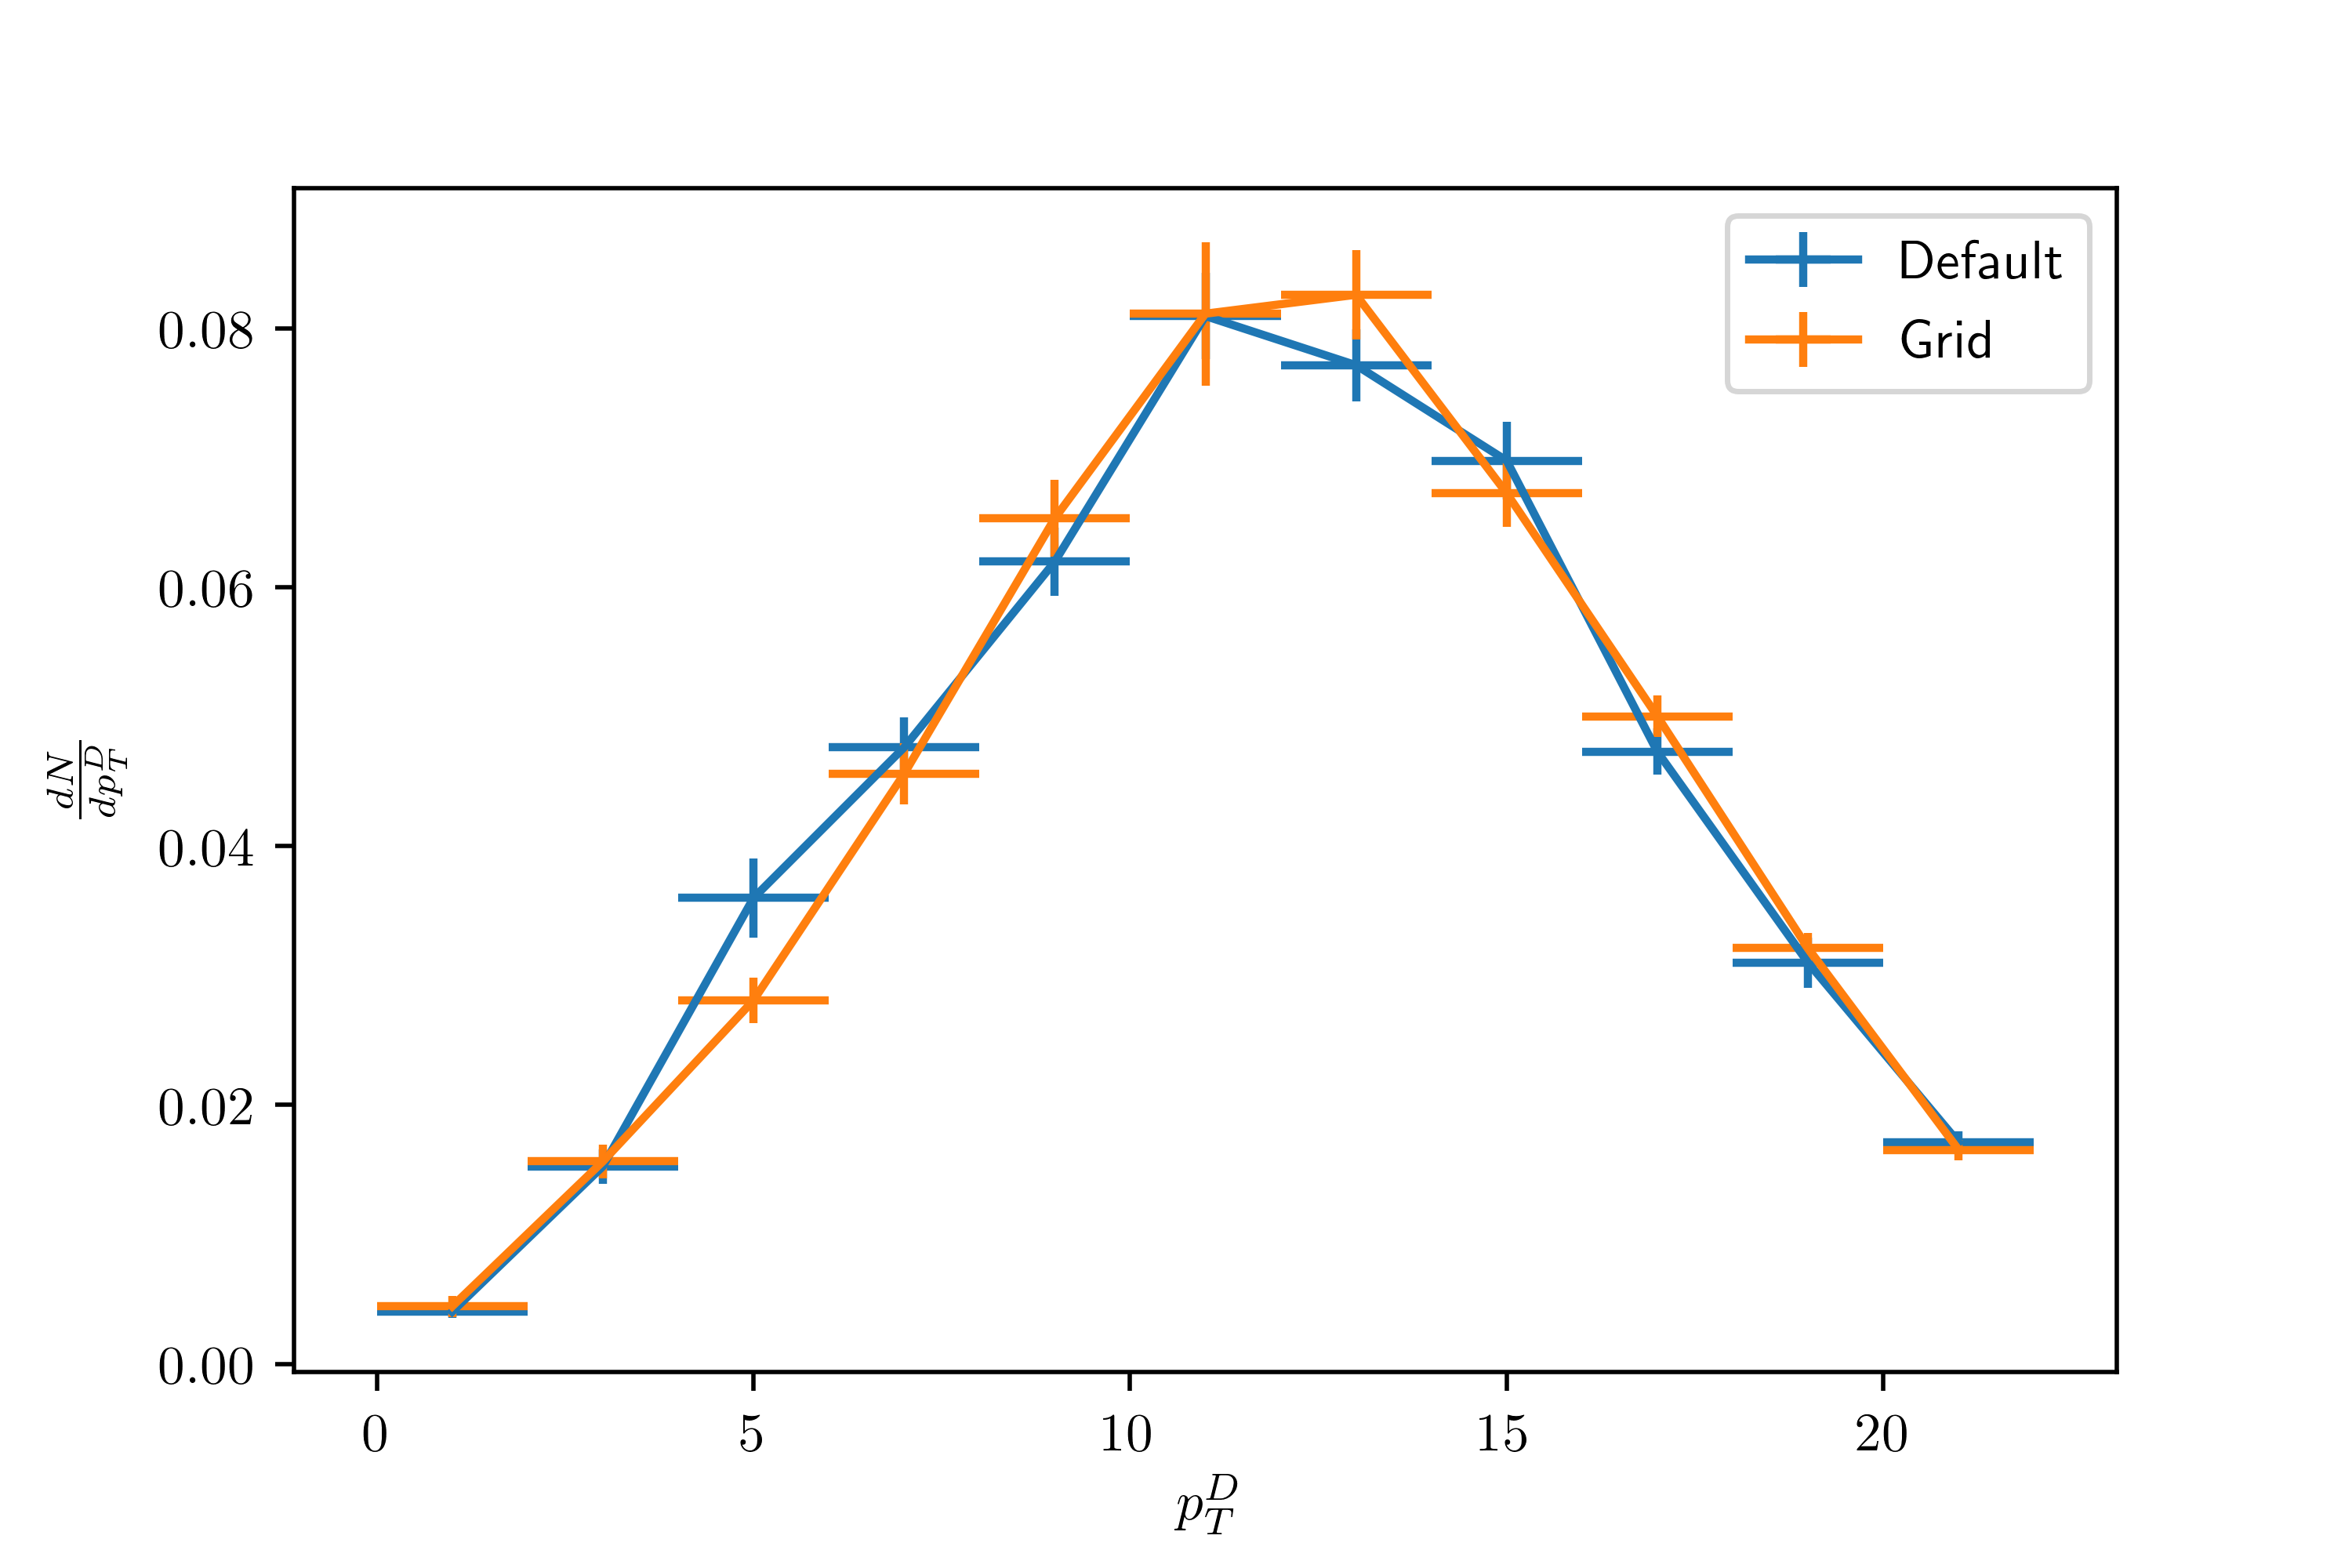
\includegraphics[width=0.7\textwidth]{images/grid_dispersion_validation.png}
\caption[Jet Dispersion for Grid validation.]{Jet Dispersion for Grid validation.}
\label{grid_dispersion_validation}
\end{figure}

\begin{figure}
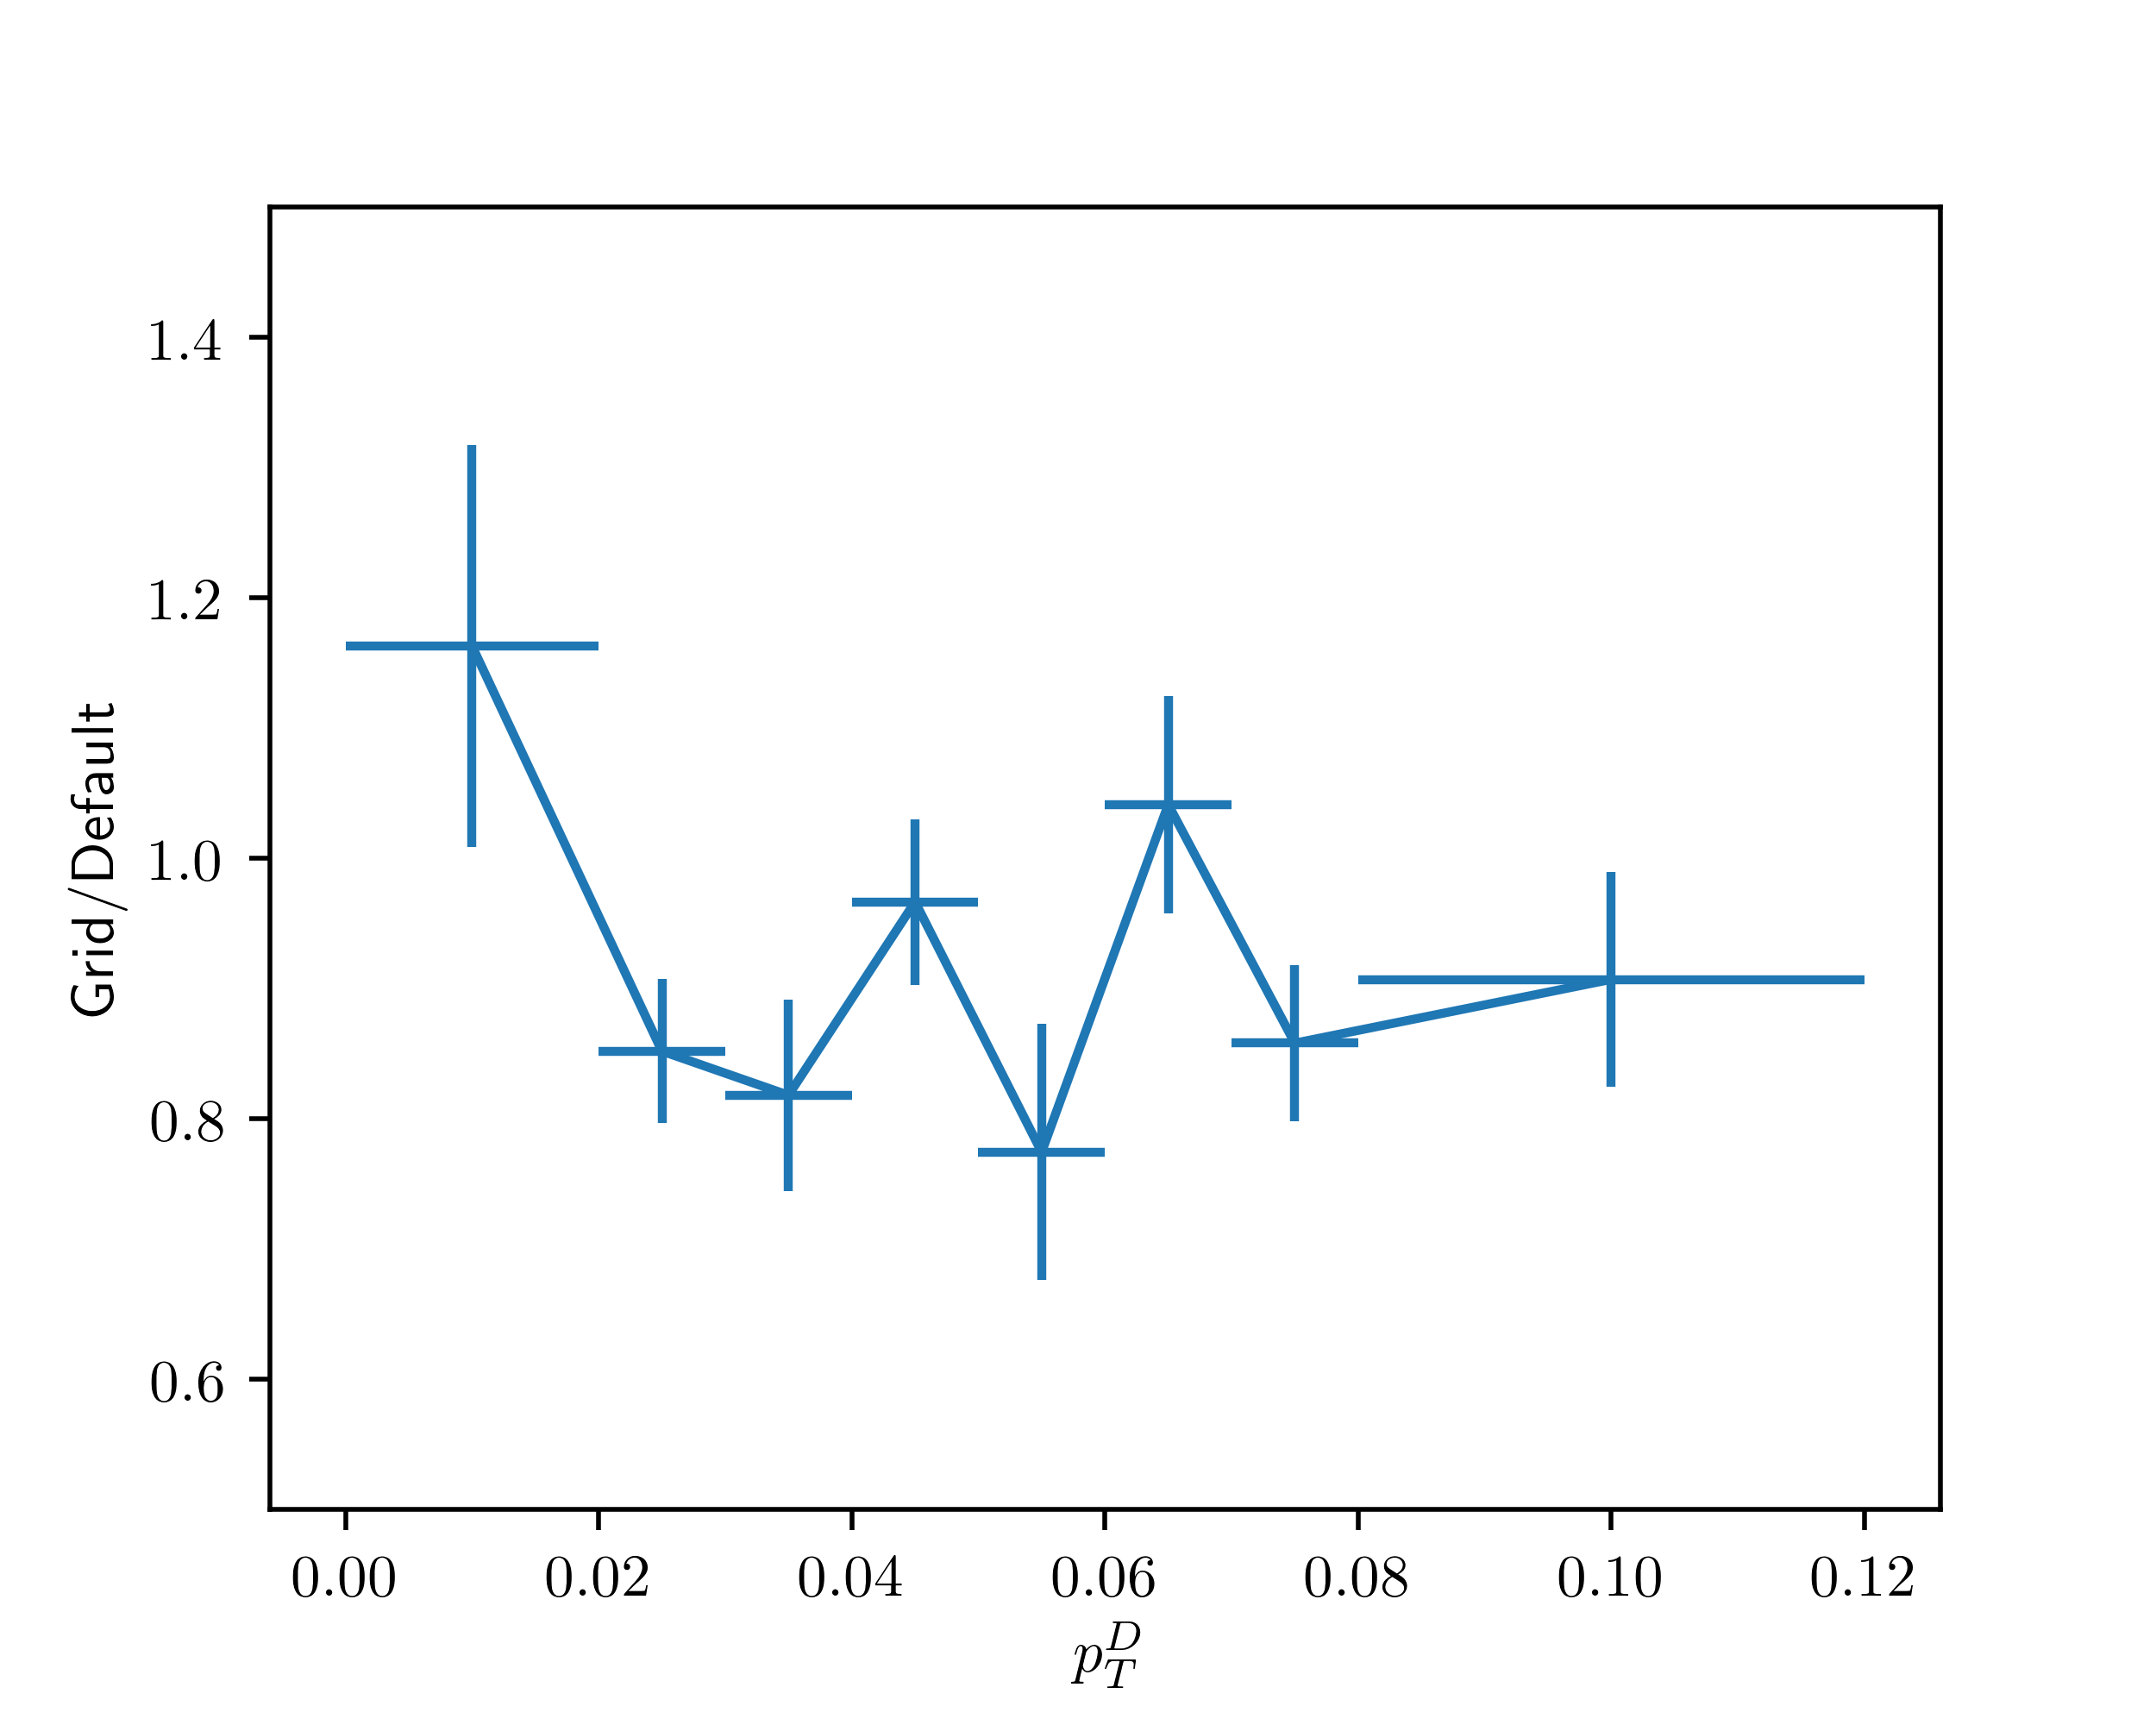
\includegraphics[width=0.7\textwidth]{images/grid_default_dispersion.png}
\caption[Grid/Default for jet dispersion]{Grid/Default for jet dispersion}
\label{grid_default_dispersion}
\end{figure}

\mychapter{Results} \label{results}
%\markboth{Resultados}{}
%\addcontentsline{toc}{chapter}{Resultados}

\mysection{Experimental Results}

Before showing the results of the simulations, it is interesting to discuss the experimental results for the studied observables. They indicate that jets suffer modifications due to interactions with the dense and hot medium created in relativistic heavy-ion collisions. The first of these, and most inclusive one is the jet $p_T$. We can observe in Figure \ref{exp_jet_pt} that the PbPb spectrum is is suppressed when compared to the pp spectrum. The same trend is observed when central and semi-peripheral collisions are compared: the former is more suppressed than the later. This indicates that there is suppression of jets for PbPb collisions, and that this suppression is also related to centrality. The fact that it varies with the centrality is also an evidence that this suppression has its origin in the interaction with the medium. In the Figure \ref{exp_jet_pt_raa} we see that the PbPb spectrum can be $20\%$ that of pp for lower transverse momentum, and saturates at no more than $60\%$ for higher values of $p_T$.

\begin{figure}
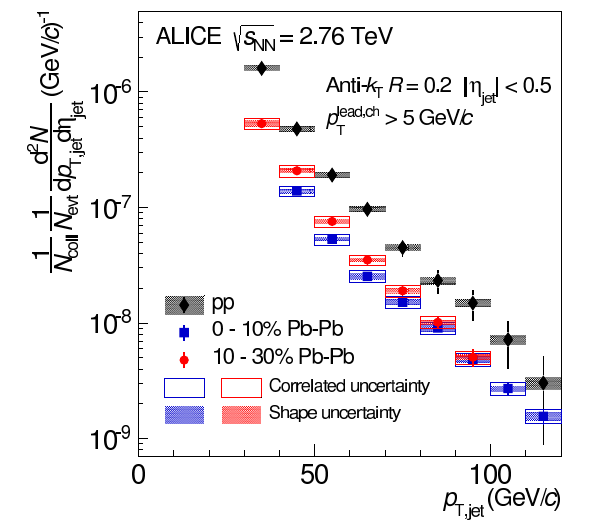
\includegraphics[width=0.6\textwidth]{images/exp_jet_pt.png}
\caption[Experimental Jet $p_T$]{The spectra of $R = 0.2$ jets with a leading track requirement of $5 \, {\rm GeV/c}$ in $0-10\%$ and $10-30\%$ most central Pb–Pb collisions scaled by $1/N_{coll}$ and in inelastic pp collisions at $\sqrt{s_{NN}} = 2.76 \, {\rm TeV}$. Plot from \cite{alice_collaboration_measurement_2015}}
\label{exp_jet_pt}
\end{figure}

\begin{figure}
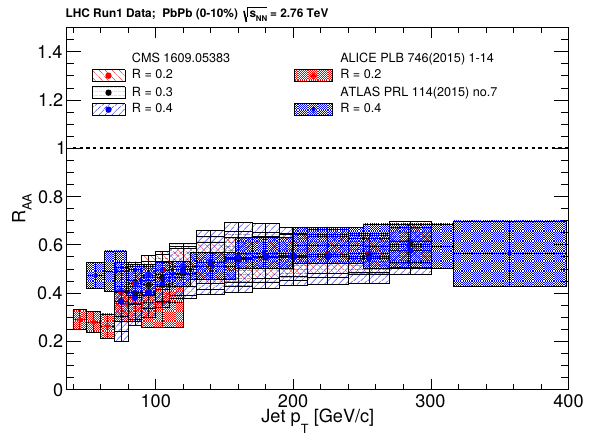
\includegraphics[width=0.6\textwidth]{images/exp_jet_pt_raa.png}
\caption[Experimental Jet $p_T$ $R_{AA}$]{Jet $p_T$ $R_{AA}$ measured in different collaborations. Figure from \cite{connors_review_2017}.}
\label{exp_jet_pt_raa}
\end{figure}

There is also evidences that this suppression is path length dependent. This can be seen in Figure \ref{exp_jet_v2} where several measurements of $v_2$ are presented. The data in orange and in white circles are measurements of the $v_2$. They come from ALICE and CMS collaborations respectively. The fact that it grows linearly for lower $p_t$ is predicted by modeling collective behavior. For $p_T \gtrsim 5\,{\rm GeV}$, the particles are not usually thermalized. The description of the particles as Jet Quenching then comes into play. We see in the plot that the $v_2$ continues to be non-zero well above $5\,{\rm GeV}$. This indicates that the energy loss of this partons must be path length dependent. The fact that it depends also on centrality is evidence that this comes from the interaction of high energy partons with the medium. The data in black circles comes and in blue squares come from ALICE and ATLAS collaborations, respectively. This data is different from the previous cases since it uses reconstructed jets. ALICE reconstructs jets with the TPC, so only charged particles are included in the analysis. ATLAS uses the hadronic calorimeters, which means it measures full jets. This difference introduces a different scale for the measurements, since ALICE will not include neutral particles when clustering the jets. For semi-central and central collisions, the collaborations do not agree upon a re-scaling of jet momenta. ALICE measures a higher value for $v_2$.

\begin{figure}
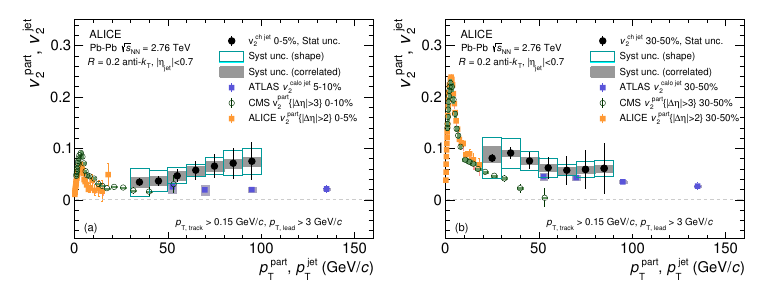
\includegraphics[width=1.0\textwidth]{images/exp_v2.png}
\caption[Experimental Jet $v_2$]{Jet $v_2$ measured in different collaborations. Figure from \cite{connors_review_2017}.}
\label{exp_jet_v2}
\end{figure}

In Figure \ref{exp_girth_ptd} we see measurements of the girth and $p_t^{D}$ for charged jets with small radius $(R=0.2)$ jets. The simulations for pp describe well the data for these observables\cite{alice_collaboration_medium_2018}. There is a modification if compared with the simulation also displayed in the plot. The girth indicates more collimated jets. The $p_t^D$ indicates harder fragmentation if compared to the pp case.

\begin{figure}
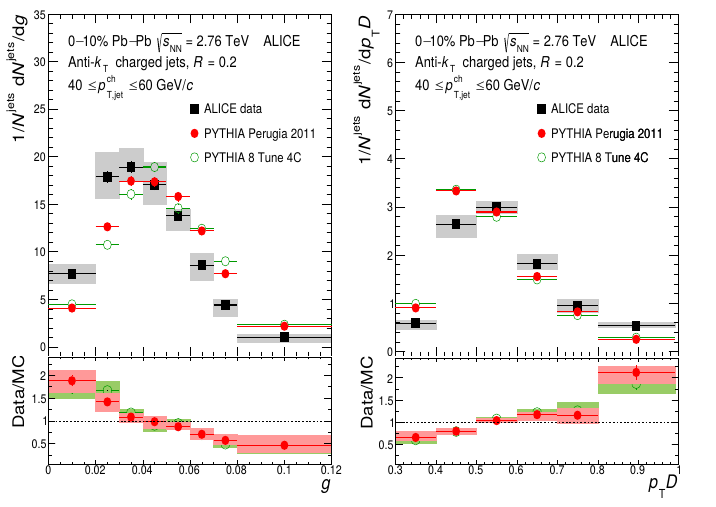
\includegraphics[width=1.0\textwidth]{images/exp_girth_ptd.png}
\caption[Experimental Girth and $p_t^{D}$]{Girth and $p_t^D$ measured by ALICE collaboration. Figure from \cite{alice_collaboration_medium_2018}.}
\label{exp_girth_ptd}
\end{figure}


Regarding jet mass, the first measurements can be seen in the Figure \ref{exp_jet_mass}. In the Figure, the mass measured in PbPb collisions is compared to pPb collisions. pp data for jet mass is well described by simulations. In \cite{alice_collaboration_first_2018} the comparison of pPb with simulations for pp show that there are no cold matter nuclear effects on this observable. So the comparison of PbPb with pPb would show only the effects of the hot QGP on the partons. For jets on the range $60-100 \, {\rm GeV}$ range, the jets in PbPb tend to have slightly lower mass than those of pPb. This indicates a broadening of the jet.

\begin{figure}
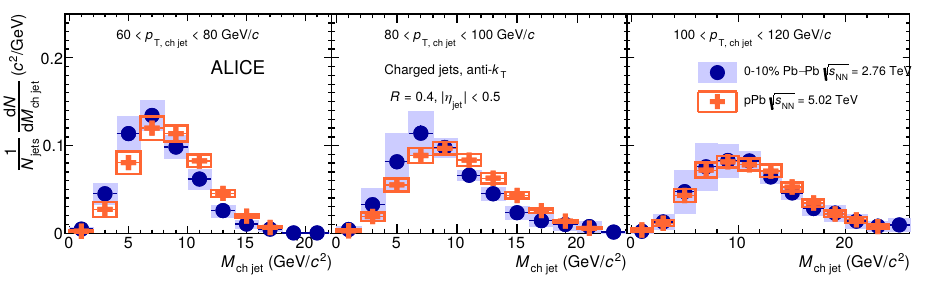
\includegraphics[width=1.0\textwidth]{images/exp_jet_mass.png}
\caption[Experimental Jet Mass]{Jet mass measured by ALICE collaboration. Figure from \cite{alice_collaboration_first_2018}.}
\label{exp_jet_mass}
\end{figure}

\mysection{JEWEL results}

JEWEL was developed to describe data from heavy-ion collisions. And it can reproduce most inclusive data. An example is displayed in Figure \ref{hadron_supression}. In the Figure we can see the prediction for neutral pion $p_t$ spectrum supression, as measured by PHENIX collaboration. It was one of the first results to indicate the phenomenum of Jet Quenching. In Figure \ref{charged_hadron_supression} we can see the supression for charged hadrons compared to data from ALICE and CMS collaborations. JEWEL describes this inclusive data really well. Also, in Figure \ref{jewel_jetpt_supression} we can see that the supression for reconstructed jets is also well described by JEWEL. The two Figures combined show that JEWEL can handle a wide energy range and different hadrochemistry well.

\begin{figure}
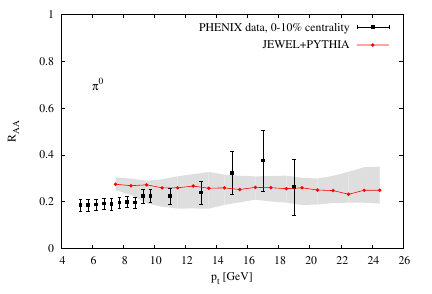
\includegraphics[width=0.8\textwidth]{images/hadron_supression.png}
\caption[Hadron $R_{AA}$]{Hadron $R_{AA}$ as measured by the PHENIX collaboration compared to JEWEL predictions. Figure from \cite{zapp_perturbative_2013}.}
\label{hadron_supression}
\end{figure}

\begin{figure}
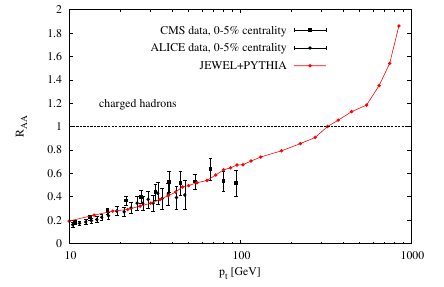
\includegraphics[width=0.8\textwidth]{images/charged_hadron_supression.png}
\caption[Charged Hadron $R_{AA}$]{Hadron $R_{AA}$ as measured by CMS and ALICE collaborations compared to JEWEL predictions. Figure from \cite{zapp_perturbative_2013}.}
\label{charged_hadron_supression}
\end{figure}

\begin{figure}
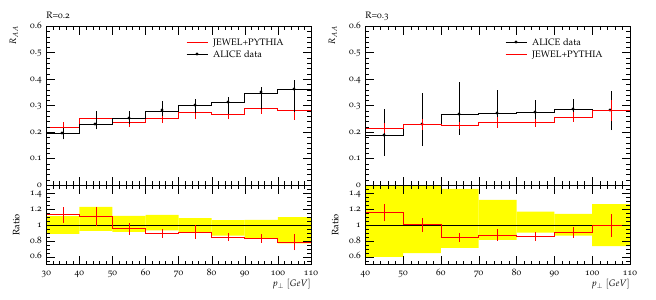
\includegraphics[width=1.0\textwidth]{images/jewel_jetpt_supression.png}
\caption[JEWEL prediction of $R_{AA}$ for the jet $p_t$.]{Jet $p_T$ $R_{AA}$ as measured by CMS, ALICE and ATLAS collaborations compared to JEWEL predictions. Figure from \cite{zapp_perturbative_2013}.}
\label{jewel_jetpt_supression}
\end{figure}

Studying internal jet structure, we can see a somewhat different picture of JEWEL performance. For instance, in Figure \ref{jewel_girth} we see that JEWEL predicts jets broader than data. In the case of jet mass, we see on Figure \ref{jewel_mass}. We are interested in this work in the case with the recoiling scattering centers, since radiation patterns trying to probe the medium is our goal. JEWEL also predicts higher values for this observable, indicating broader jets than expected. In the case without recoils, the jet mass has lower values than data, which indicates a hardening of the core.

\begin{figure}
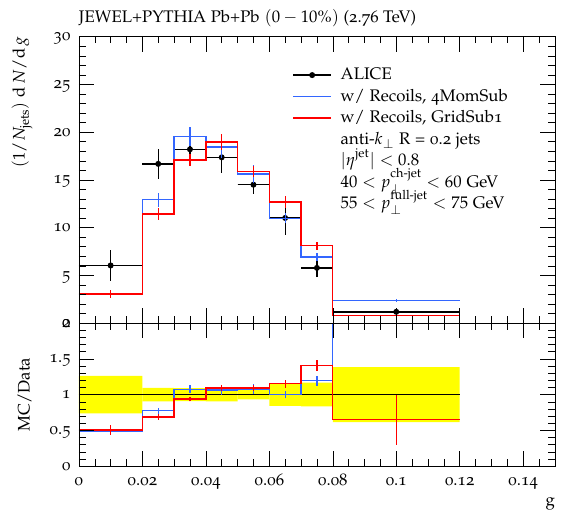
\includegraphics[width=1.0\textwidth]{images/jewel_girth.png}
\caption[JEWEL prediction for girth.]{JEWEL predictions for jet girth compared to measurements from ALICE collaboration. Figure from \cite{elayavalli_medium_2017}.}
\label{jewel_girth}
\end{figure}

\begin{figure}
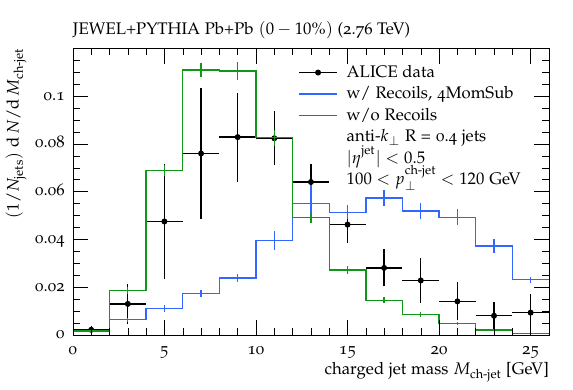
\includegraphics[width=1.0\textwidth]{images/jewel_mass.png}
\caption[JEWEL prediction for mass.]{JEWEL predictions for jet mass compared to measurements from ALICE collaboration. Figure from \cite{elayavalli_medium_2017}.}
\label{jewel_mass}
\end{figure}

\mysection{JEWEL with realistic IC} \label{jewel_with_ic}

In Figure \ref{jet_girth_ic} we see the results for jet girth with realistic initial conditions. Here $\rm T_RENTo$ was used with calibration to fit IP-Glasma results\cite{moreland_alternative_2015}. JEWEL tends to overestimate the peak value even with the new initial conditions. One is reminded that girth is related to the angular opening of the jet. Girth also depends linearly on the transverse momenta of the particles. The overestimation of JEWEL results tells us that the jets produced by the simulation tend to be slightly broader than the jets from data. No further improvement comes from the inclusion of more realistic initial conditions, as the results given by the inclusion of realistic initial conditions agree with the default of JEWEL.

\begin{figure}
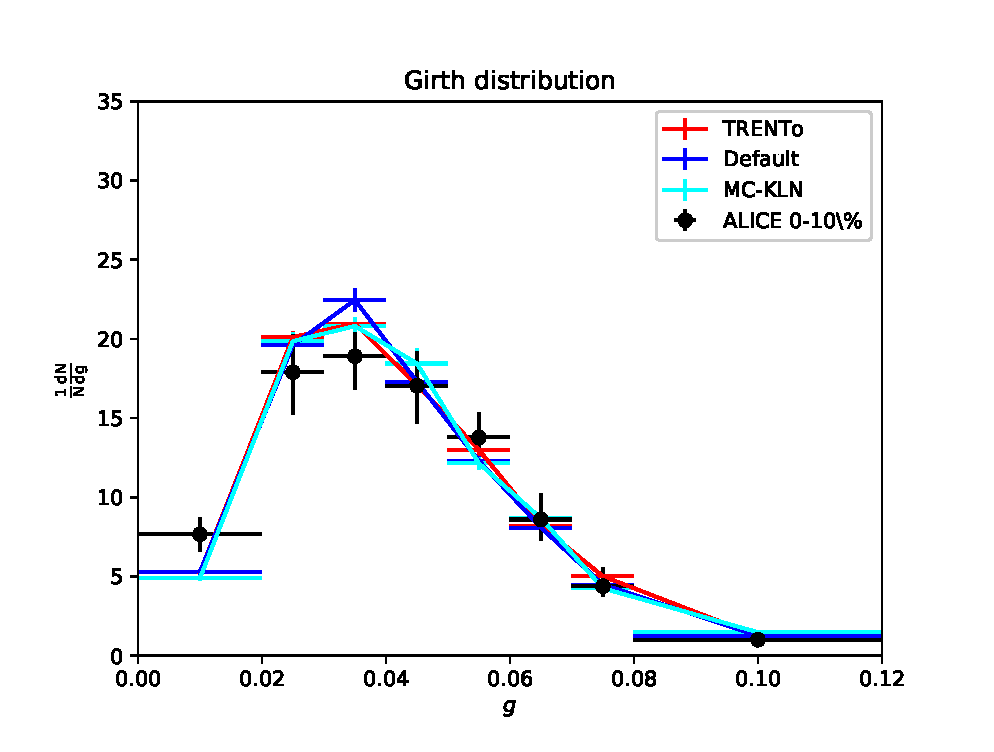
\includegraphics[width=1.0\textwidth]{images/My_Angularity_3.eps}
\caption[Jet Girth with realistic IC]{Jet Girth for charged jets calculated for $R=0.2$ anti-kt algorithm and $|\eta|<0.8$. $40 {\rm GeV/c} < p_T < 60 {\rm GeV}$. The CM energy is $\sqrt{s_{NN}}= 2.76 {\rm TeV}$. On the $0-10\%$ centrality class.}
\label{jet_girth_ic}
\end{figure}

In Figure \ref{jet_dispersion_ic} we see the results for the jet dispersion. The default of JEWEl predicts slightly lower values than data. This indicates softer fragmentation. With the inclusion of realistic initial conditions, there is no substantial difference.

\begin{figure}
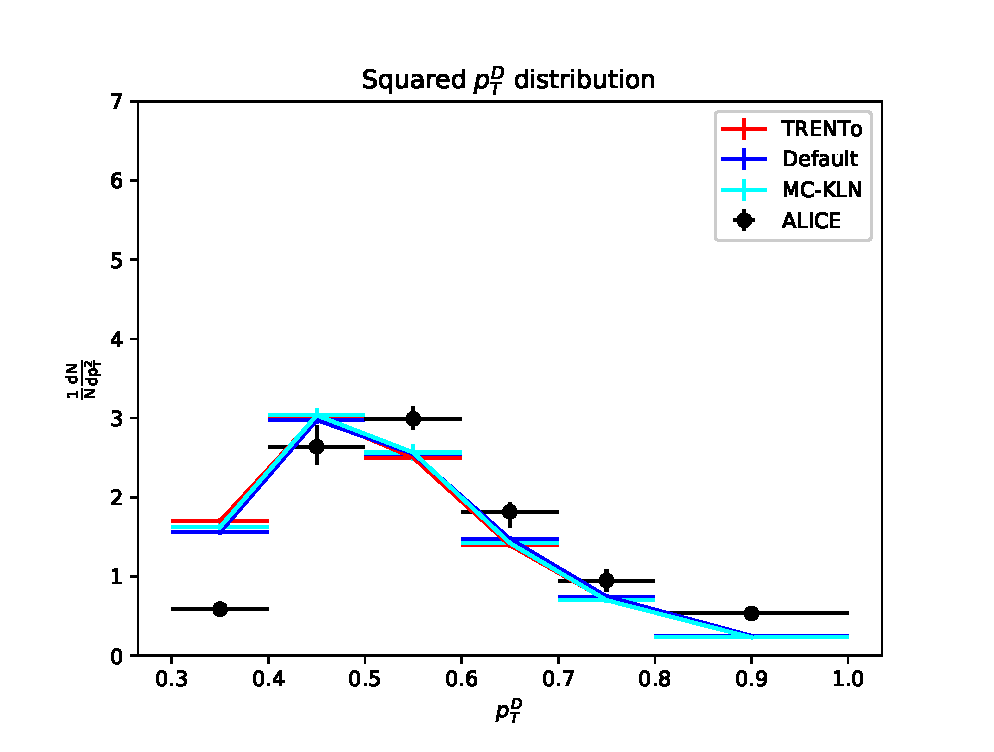
\includegraphics[width=1.0\textwidth]{images/Squared_3.eps}
\caption[Jet $p_D^T$ with realistic IC]{Jet Dispersion for charged jets calculated for $R=0.2$ anti-kt algorithm and $|\eta|<0.8$. $40 {\rm GeV/c} < p_T < 60 {\rm GeV}$. The CM energy is $\sqrt{s_{NN}}= 2.76 {\rm TeV}$. On the $0-10\%$ centrality class.}
\label{jet_dispersion_ic}
\end{figure}

The results for the jet mass are displayed in Figure \ref{jet_mass_ic}. Here we present also the inclusion of realistic IC for this observable. JEWEL in its default does not make a good prediction for it already. The problem is of the same nature of the disagreement of the girth, but worst. The jets in data tend to have a lower mass than predicted, this indicates larger jets, as is the case with girth. The mass further indicates that the problem lies in the soft fragmentation, which depends strongly on hadronization. There is some improvement from the addition of the realistic IC background, as one can see from the slight shift to the left. This shift is not significant though, due to the uncertainties of the method. There is a discrepancy in the spectrum. 

\begin{figure}
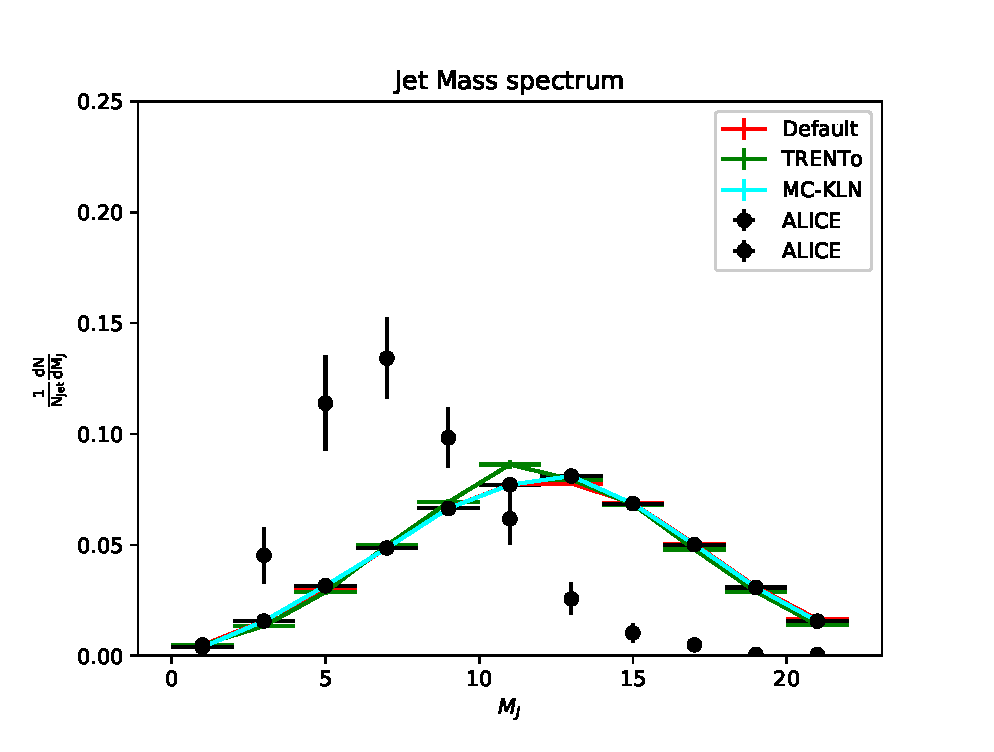
\includegraphics[width=1.0\textwidth]{images/Mass_3.eps}
\caption[Jet Mass with realistic IC]{Jet Mass for charged jets calculated for $R=0.2$ anti-kt algorithm and $|\eta|<0.8$. $40 {\rm GeV/c} < p_T < 60 {\rm GeV}$. The CM energy is $\sqrt{s_{NN}}= 2.76 {\rm TeV}$. On the $0-10\%$ centrality class.}
\label{jet_mass_ic}
\end{figure}

In Figure \ref{jet_v2_ic} we see the results for the jet $v_2$. The data from ALICE and ATLAS show that there is tension between the experimental results making any conclusion about the performance of the model more difficult. ALICE uses their TPCs for jet reconstruction and ATLAS uses the hadronic calorimeters. This means that ALICE uses only charged particles, and ATLAS uses all hadrons for jet reconstruction. This explains why ALICE data has lower values of $p_T$. Although there is a disagreement between the collaborations, both data seems to indicate that the $v_2$ is different from zero. This is expected from fluctuations that happen on the initial conditions, since central collisions don't have a geometry that naturally raises an azimuthal asymmetry on the energy distribution. We can see in the Figure \ref{jet_v2_ic} that JEWEL, even with realistic IC, predicts values consistent with zero $v_2$.

\begin{figure}
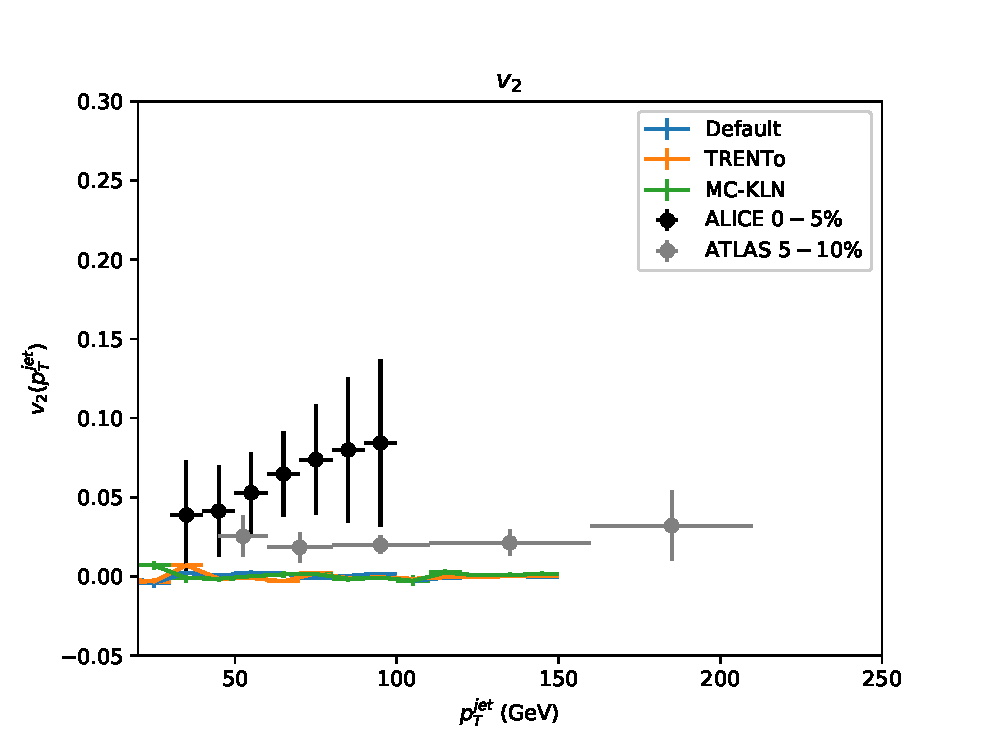
\includegraphics[width=1.0\textwidth]{images/v2_4.eps}
\caption[Jet $v_2$ with realistic IC]{Jet $v_2$ calculated for $R=0.4$ anti-kt algorithm and $|\eta|<0.8$. The CM energy is $\sqrt{s_{NN}}= 2.76 {\rm TeV}$. On the $0-10\%$ centrality class.}
\label{jet_v2_ic}
\end{figure}

\mysection{JEWEL with realistic hydro} \label{jewel_with_hydro}

In Figure \ref{jet_girth} we see the results for jet girth. Considering the hydrodynamic expansion for the medium as well. The result shows that JEWEL tends to overestimate it. Since girth is related to the jet width, this shows broader jets than the data. No further improvement comes from the inclusion of more realistic initial conditions or hydrodynamics, as the results given by the inclusion of the realistic hydro and initial conditions agree with the default of JEWEL.

\begin{figure}
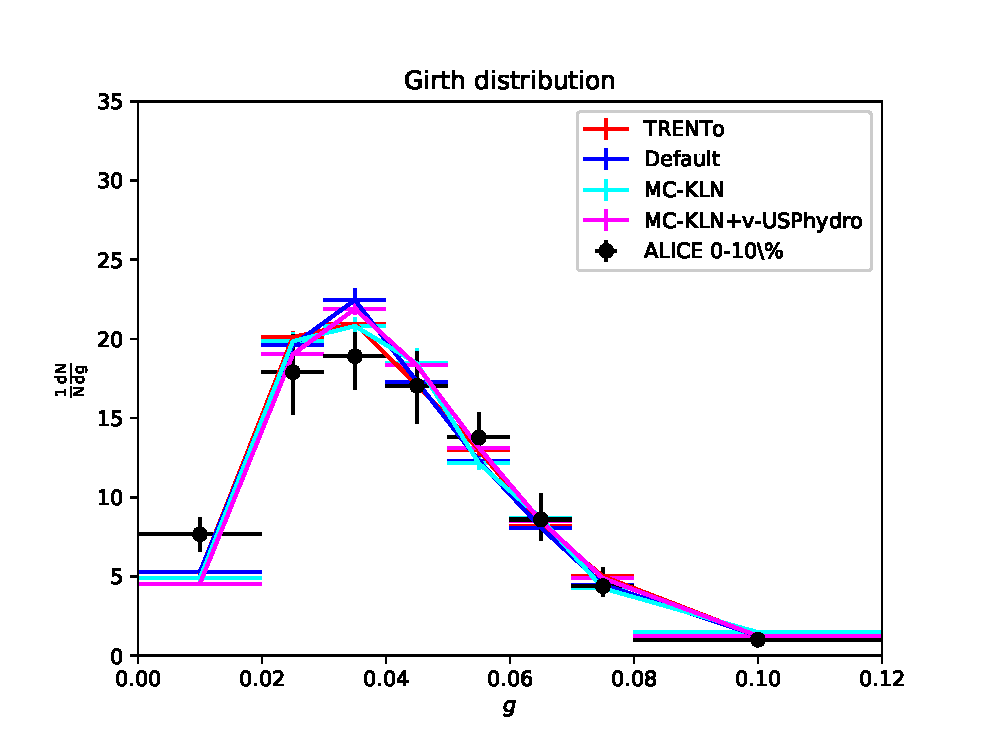
\includegraphics[width=1.0\textwidth]{images/My_Angularity_4.eps}
\caption[Jet Girth]{Jet Girth for charged jets calculated for $R=0.2$ anti-kt algorithm and $|\eta|<0.8$. $40 {\rm GeV/c} < p_T < 60 {\rm GeV}$. The CM energy is $\sqrt{s_{NN}}= 2.76 {\rm TeV}$. On the $0-10\%$ centrality class.}
\label{jet_girth}
\end{figure}

In Figure \ref{jet_dispersion} we see the results for the jet dispersion with the inclusion of realistic hydro. The default of JEWEl predicts slightly lower values than data. This indicates softer fragmentation. With the inclusion of realistic hydro, the agreement is slightly worst for lower values, but not substantially different. This indicates that the fragmentation is slightly softer than that of the default. Regions of greater density on the profile could be responsible for the further soft radiation causing this.

\begin{figure}
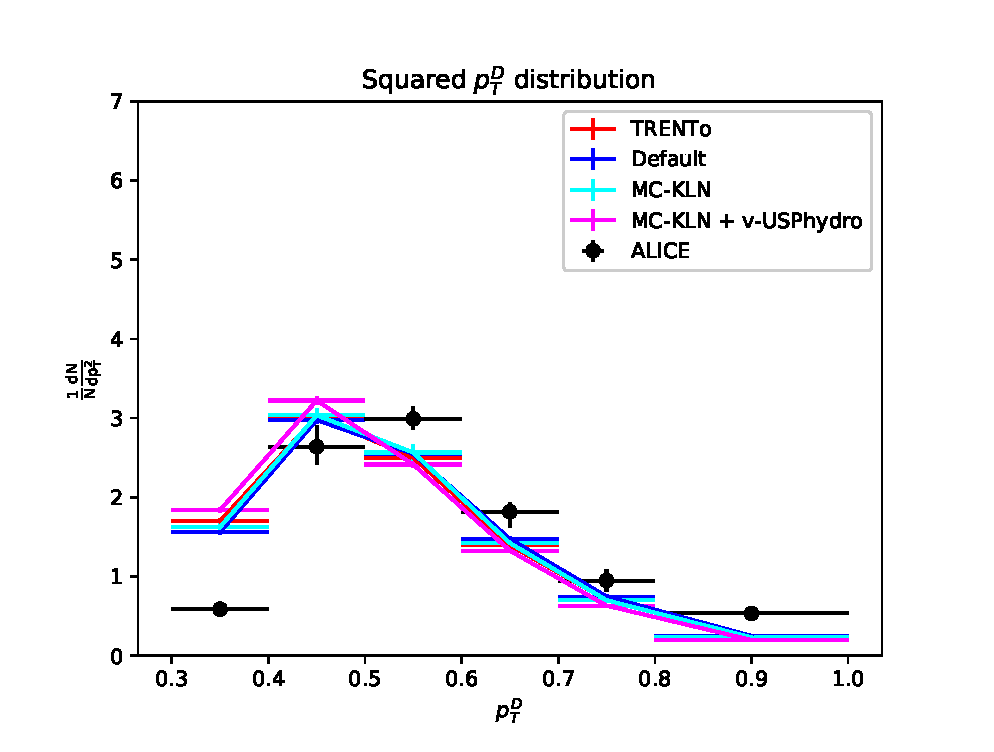
\includegraphics[width=1.0\textwidth]{images/Squared_4.eps}
\caption[Jet $p_D^T$]{Jet Dispersion for charged jets calculated for $R=0.2$ anti-kt algorithm and $|\eta|<0.8$. $40 {\rm GeV/c} < p_T < 60 {\rm GeV}$. The CM energy is $\sqrt{s_{NN}}= 2.76 {\rm TeV}$. On the $0-10\%$ centrality class.}
\label{jet_dispersion}
\end{figure}

The results for the jet mass are displayed in Figure \ref{jet_mass}. JEWEL in its default doesn't make a good prediction for it. The problem is of the same nature of the disagreement of the girth, but worst. The jets in data tend to have a lower mass than predicted, this indicates larger jets, as is the case with girth. The mass further indicates that the problem lies in the soft fragmentation, which depends strongly on hadronization. There is some improvement from the addition of the realistic hydrodynamics background, although there is a discrepancy in the spectrum. 

\begin{figure}
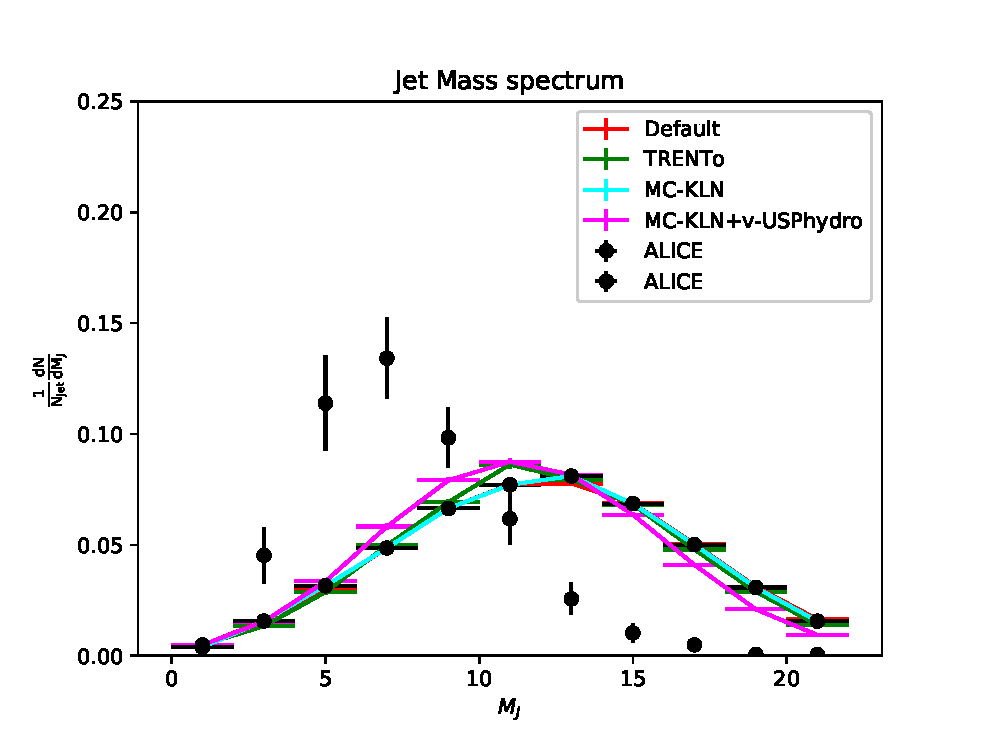
\includegraphics[width=1.0\textwidth]{images/Mass_4.eps}
\caption[Jet Mass]{Jet Mass for charged jets calculated for $R=0.2$ anti-kt algorithm and $|\eta|<0.8$. $40 {\rm GeV/c} < p_T < 60 {\rm GeV}$. The CM energy is $\sqrt{s_{NN}}= 2.76 {\rm TeV}$. On the $0-10\%$ centrality class.}
\label{jet_mass}
\end{figure}

In Figure \ref{jet_v2} we see the results for the jet $v_2$, with the inclusion of realistic hydro. Although there is a disagreement between the collaborations, both data seems to indicate that the $v_2$ is different from zero. The fluctuations might be responsible for the existence of the asymmetry. We can see in Figure \ref{jet_v2} that the inclusion of the realistic hydro has raised the $v_2$ from zero, although there seems to be overestimating it. The simulations currently performed tell us that the combined effect of realistic initial conditions and hydrodynamics are responsible for this effect. The fact that neither MC-KLN nor $\rm T_RENTo$ have shown significant $v_2$ indicates that the hydrodynamics is an essential ingredient for describing this observable.

\begin{figure}
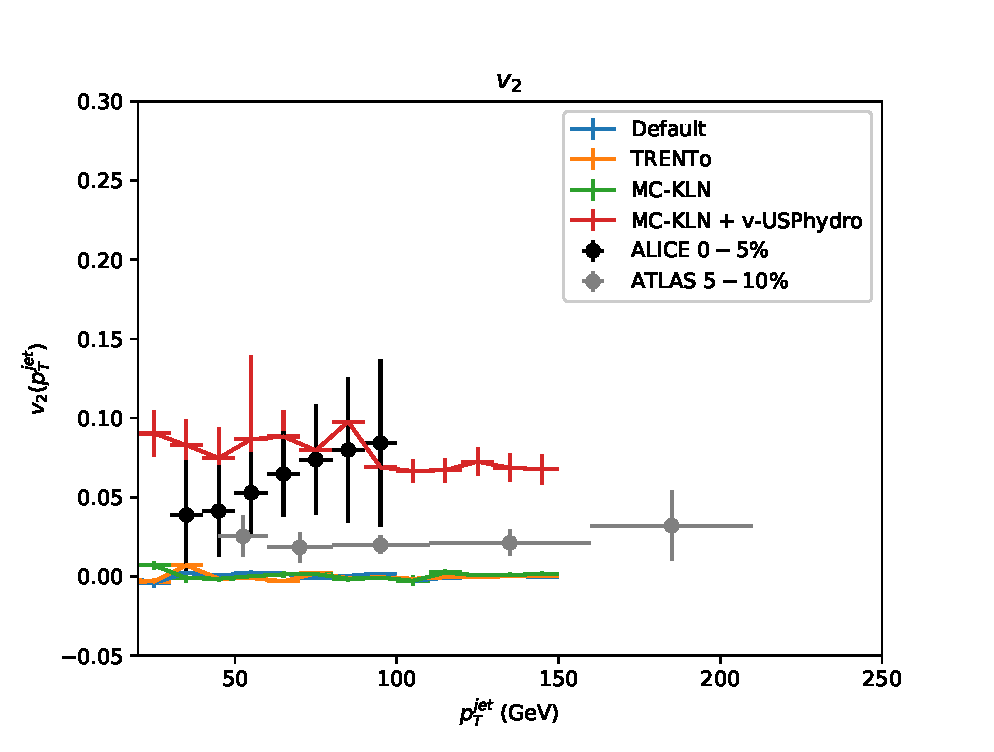
\includegraphics[width=1.0\textwidth]{images/v2_5.eps}
\caption[Jet $v_2$]{Jet $v_2$ calculated for $R=0.4$ anti-kt algorithm and $|\eta|<0.8$. The CM energy is $\sqrt{s_{NN}}= 2.76 {\rm TeV}$. On the $0-10\%$ centrality class.}
\label{jet_v2}
\end{figure}

\mychapter{Conclusion} \label{conclusions}
%\markboth{Conclusão}{}
%\addcontentsline{toc}{chapter}{Conclusão}

The results presented in the previous chapter show that, as far as the jet structure and shape are concerned, there are no major modifications of the observables due to the inclusion of realistic hydro and initial conditions. Some improvements came on the jet mass, bit only slightly.
\par
To improve the description of the data, other things could be modified. First, there is still the hadronization mechanism that is used by JEWEL, which comes from PYTHIA. This mechanism is built to explain pp data. Jets formed in heavy-ion collisions might be substantially different due to their hadronization mechanism. Effects of coalescence might play a big role here, giving new color partners to the leading partons describing the jets.
\par
Another thing that was not implemented in this work is the local four-velocity and a realistic EOS. This could further improve the description of the data. Since the partons are moving through the medium and the medium itself is most of the time moving outwards, the collisions could be more collinear than JEWEL default predicts. This could collimate the jet further, resulting in narrower jets. The collisions would be softer as well, since the CM of the local elastic collisions would be smaller, perhaps resulting in harder hadrons in the center of the jets in the final state. This could improve the $p_T^D$ data as well.
\par
The sample of the results presented in this work shows that there is not, as far as internal jet substructure and shape is concerned, a major improvement in describing the observables by implementing more realistic initial conditions or realistic hydrodynamics. Also, the correlation between medium and jets does present modifications due to the inclusion of a more realistic background, as indicated in the $v_2$ results. There is still high uncertainty in the experimental data, and further experimental improvement is needed for more detailed comparisons. The fact that this observable showed a value different from zero does indicate that high energy partons can be used to investigate properties of the medium through this kind of observable. Further information can be potentially extracted from the medium by looking at higher moments of the Fourier decomposition. This can aid in constraining the models applied in these predictions, as well as extract the transport coefficients from the QGP.

\bibliography{Bibliografia/bibliography.bib}
\markboth{Bibliography}{}
%\bibliographystyle{IEEEtran}
\bibliographystyle{ieeetr}

\printindex

\end{document}